\documentclass[winfonts,UTF8,a4paper]{ctexart}
%%package
\usepackage{url}
\usepackage[lined,boxruled,commentsnumbered]{algorithm2e}
\usepackage{amsfonts}
\usepackage[figurewithin=section]{caption}
\usepackage{color}
\usepackage{fancyhdr}
\usepackage{floatrow}
\usepackage[text={160mm,247mm},left=30mm,right=20mm,includeheadfoot,vmarginratio=1:1]{geometry}
\usepackage{graphicx}
\usepackage{amsmath}
\usepackage{algorithmic}
\usepackage{array}
\usepackage{fixltx2e}
\usepackage{stfloats}
\usepackage{url}
\usepackage{multicol}
\usepackage{graphicx}
\usepackage{ctex}
\usepackage{subfigure}
\usepackage{float}
\usepackage{indentfirst}
\usepackage{booktabs}
\usepackage{lscape}
\usepackage{caption}
\usepackage{xcolor}  
\usepackage{tikz}  
\usepackage{tikz,mathpazo}

\usepackage[numbers,sort&compress]{natbib}
\usepackage{setspace}
\usepackage{tabularx}
\graphicspath{{graph/}}

%重设Code环境

%%参数设置
\onehalfspacing %%1.5倍行距
\renewcommand{\footnotesize}{\zihao{5}}%%设置脚注字号
\floatsetup[table]{capposition=top}%%表格标题在表格上方
%页眉,页脚
\pagestyle{fancy}
\fancyhf{}
\fancyhead[C]{\zihao{-5} 暨南大学本科毕业设计(论文)}


\CTEXsetup[name={,},number={\arabic{section}},format={\zihao{-2}\bf},nameformat={\songti\zihao{-2}\bf},aftername={\ }]{section}
\CTEXsetup[name={,},number={\arabic{section}.\arabic{subsection}},
format={\zihao{4}\bf},nameformat={\songti\zihao{4}\bf},aftername={\ }]{subsection}
\CTEXsetup[name={,},number={\arabic{section}.\arabic{subsection}.\arabic{subsubsection}},
format={\zihao{4}\bf},nameformat={\songti\zihao{4}\bf},aftername={\ }]{subsubsection}
\CTEXsetup[name={,},number={\arabic{section}.\arabic{subsection}.\arabic{subsubsection}.\arabic{paragraph}},
format={\zihao{4}\bf},nameformat={\songti\zihao{4}\bf},aftername={\ }]{paragraph}
\CTEXsetup[name={,},number={\arabic{section}.\arabic{subsection}.\arabic{subsubsection}.\arabic{paragraph}.\arabic{subparagraph}},
format={\zihao{4}\bf},nameformat={\songti\zihao{4}\bf},aftername={\ }]{subparagraph}

%重设图片、表格标号
\makeatletter
    \renewcommand{\thefigure}{\ifnum \c@section>\z@ \thesection-\fi \@arabic\c@figure}
    \renewcommand{\thetable}{\ifnum \c@section>\z@ \thesection-\fi \@arabic\c@table}
    \renewcommand{\theequation}{式\  \ifnum \c@section>\z@ \thesection-\fi \@arabic\c@equation}
\makeatother
%重设目录格式
\usepackage{titletoc}


\titlecontents{section}[1em]{\addvspace{.3em}\bfseries}{\contentslabel{1em}}{}
{\ \titlerule*[5pt]{$\cdot$}\contentspage}[\addvspace{.3em}]
\titlecontents{subsection}[2.8em]{}{\contentslabel{1.8em}}{}{\ \titlerule*[5pt]{$\cdot$}\contentspage}
\titlecontents{subsubsection}[4.6em]{}{\contentslabel{2.6em}}{}{\ \titlerule*[5pt]{$\cdot$}\contentspage}


\usepackage{hyperref}
\hypersetup{colorlinks=true,linkcolor=black}
\newcommand{\upcite}[1]{{\textsuperscript{\cite{#1}}}}
%\newcommand{\upcite}[1]{\textsuperscript{\textsuperscript{\cite{#1}}}}
\usepackage{subfigure}
%不需要使用gbt7714,已将gbt7714放入根目录
%\usepackage{gbt7714}

\usepackage{tikz}
\usetikzlibrary{positioning, shapes.geometric}
\usetikzlibrary{calc}

\tikzstyle{format}=[rectangle,draw,thin,fill=white]  
%定义语句块的颜色,形状和边
\tikzstyle{test}=[diamond,aspect=2,draw,thin]  
%定义条件块的形状,颜色
\tikzstyle{point}=[coordinate,on grid,]  
\tikzstyle{startstop} = [rectangle, rounded corners,minimum height=0.7cm,text centered, draw=black]
\tikzstyle{io} = [trapezium, trapezium left angle=70, trapezium right angle=110,  minimum height=0.7cm, text centered, draw=black]
\tikzstyle{process} = [rectangle,  minimum height=0.7cm, text centered, draw=black]
\tikzstyle{decision} = [diamond, minimum height=0.7cm, text centered, draw=black]
\tikzstyle{arrow} = [thick,->,>=stealth]
\tikzstyle{every node}=[font=\normalsize]


\usepackage{listings}
\usepackage{xcolor} 
\makeatletter
\renewcommand{\maketag@@@}[1]{\hbox{\m@th\normalsize\normalfont#1}}%
\makeatother

\definecolor{mygreen}{rgb}{0,0.6,0}
\definecolor{mygray}{rgb}{0.5,0.5,0.5}
\definecolor{mymauve}{rgb}{0.58,0,0.82}
\lstset{ %
	backgroundcolor=\color{white},   % choose the background color
	basicstyle=\footnotesize\ttfamily,        % size of fonts used for the code
	columns=fullflexible,
	breaklines=true,                 % automatic line breaking only at whitespace
	captionpos=b,                    % sets the caption-position to bottom
	tabsize=4,
	commentstyle=\color{mygreen},    % comment style
	escapeinside={\%*}{*)},          % if you want to add LaTeX within your code
	keywordstyle=\color{blue},       % keyword style
	stringstyle=\color{mymauve}\ttfamily,     % string literal style
	frame=shadowbox,
	rulesepcolor=\color{red!20!green!20!blue!20},
	% identifierstyle=\color{red},
	numbers=left, 
	numberstyle=\tiny,
	% escapeinside=' ',
	xleftmargin=2em,
	xrightmargin=2em, 
	aboveskip=1em
}
\usepackage{hyperref}
\hypersetup{colorlinks=true,linkcolor=black,citecolor=black}




\begin{document}
  %%--------------- 前言 ----------------- %%
    \begin{center}
  \zihao{2}\textbf{\kaishu 诚 ~~ 信 ~~ 声 ~~ 明}
\end{center}\par
\vspace{10mm}
\zihao{-3}
\kaishu
我声明,所呈交的课程论文是本人在老师指导下进行的研究工作及取得的研究成果。据我查证,除了文中特别加以标注和致谢的地方外,论文中不包含其他人已经发表或撰写过的研究成果,也不包含为获得其他教育机构的学位或证书而使用过的材料。我承诺,论文中的所有内容均真实、可信。\\[45mm]
课程论文作者签名:\hspace{30mm}签名日期:\qquad 年\quad 月\quad 日
\newpage

    \songti
\begin{center}
  \zihao{-2}\textbf{电力系统网源协调控制系统开发}
\end{center}
\vspace{0.5cm}\noindent\textbf{[摘要]\quad}
在如今的电力市场和大力发展新能源电力、大量分布式、小容量新能源机组需要并网的环境下,网源协调的问题日益突出。良好的网源协调能力对电力系统运行有着极大的作用。然而现有的网源协调分析和控制方法主要用于集中式、大容量机组,针对小容量、分布式并网主体(如风力发电、光伏发电等)的应用尚不成熟。本文根据《南方区域“两个细则”》以及《南方区域“两个细则”修订内容》,结合小容量、分布式并网主体自身的特点,提出了对应的考核制度,并为其提供一个通用性的考核平台框架。
通过该平台可以实时可视化分析并网主体的网源协调种指标,从改善电厂发电、调频调峰以及出力策略等方面为改善并网主体的网源协调动作提供优化方案,进一步改善该类机组的网源协调问题。

%系统等方面出发,可视化显示多种指标体系,
%
%构建以新能源为主体的新型电力系统是我国2030年前实现碳达峰、2060年前实现碳中和的关键。针对风光等新能源机组存在等效转动惯量很小、缺乏相关频率调节功能及电压调节能力有限等缺点危害系统安全稳定运行的难题,可考虑开展新型电力系统网源协调分析与控制研究。然而,现有的网源协调分析与控制方法主要用于集中式、大容量的机组,尚未有研究将该分析与控制方法直接应用于分布式、小容量的并网主体(如风电、光伏、虚拟电厂等)上。为此,本项目计划:研究适用于分布式小容量并网主体的网源协调分析方法、研究适用于分布式小容量并网主体的网源协调控制方法、以及建设适用于分布式小容量并网主体网源协调分析与控制的通用性平台。项目研究成果将构建并网主体网源协调问题的分析与控制理论并形成一个适用于分布式小容量并网主体网源协调分析与控制的通用性平台,通过该平台可实时分析各并网主体的网源协调动作情况、可设计控制器优化各并网主体的网源协调动作使其满足并网要求。
\par\vspace{1cm}\noindent\textbf{[关键词]\quad}
\textbf{电力系统;网源协调;两个细则;一次调频;新能源功率预测}
\newpage

%English Abstract
\begin{center}
  \zihao{-2}\textbf{Development of Power System Grid-Ssource Coordination Control System}
\end{center}
\vspace{0.5cm}\noindent\textbf{\bf{Abstract}\quad}
Today, in the environment of the electricity market and a large number of distributed small capacity new energy generator sets that needed to be connected to the grid, the problem of gird-source coordination is much more serious than ever before. The gird-source coordination plays a great role in the operation of the power systerm. However, the existing gird-source coordination analysis and control methods are mainly designed for centralized and high-capacity generator sets. The application for those smaller and diastrbuted sets, such as wind power and photovoltaics, is immature. According to \textit{the Two Rules of the Southern Region} and \textit{the Revised Contents of the Two Rules of the Southern Region}, and in consideration of the characteristics of these generator sets, this paper puts forward the corresponding assessment system and provides a universal platform framework. The system visually displays a variety of indexs in order to provide a suggestion to improve the coordinated development of the Grid and the Source. Therefore it might helps to the problem of gird-source coordination.
\par\vspace{1cm}\noindent\textbf{Keywords\quad}
\textbf{Electrical Power System; Grid-Source Coordination; the \textit{Two Rules}; the Primary Frequency Modulation; New Energy Power Forecast}


    \zihao{4}
    \tableofcontents
 \thispagestyle{empty}
 \newpage

%%----------------- 正文设置 ----------------- %%

%重设页眉,页脚
\pagestyle{fancy}
\fancyhf{}
\fancyhead[C]{\zihao{-5} 电厂辅助服务分析支撑演示平台开发}
\fancyfoot[R]{\thepage}
%重设页码
\setcounter{page}{1}
\pagenumbering{arabic}
%-------------正文----------%
\newpage
\section{绪论}
\subsection{研究背景与现状}
近年来,风力发电、光伏发电等新能源发电技术日益成熟\upcite{田皓2021基于趋势理论的源},分布式小规模新能源机组并网比例日益增大\upcite{陈锴2020考虑输电断面限制的风,宋杰2021蓄热式电采暖负荷参与风电消纳运行策略研究}。针对风力、光伏等新能源机组,由于其能量来源具有随机性与不确定性\upcite{高阳2010基于噪声场合下},若将该类机组直接并网,则会对电网电能质量带来较大的影响,比如:影响电网频率和电压波动、对谐波产生影响等\upcite{郭俊飞2015探讨风电场并网运行对电网电能质量的影响}。因此使得网-源-荷间的协调发展问题变得尤为突出。

对于网源协调的问题,传统解决办法大致可以归为两种。其一是使用补偿装置,如静止无功补偿装置、静止同步补偿器等\upcite{田广青1995静止无功补偿技术与应用,田广青1996静止无功补偿技术与应用}。其二是使用储能技术\upcite{周皓2021改善风电并网电能质量的飞轮储能系统能量管理系统设计,张维煜2014飞轮储能关键技术及其发展现状,李军徽201810,沈冠冶2018考虑风电并网系统的储能优化配置},如飞轮储能、锂电池储能、海水蓄能、压缩空气储能等。但如上方法都需要使用外置设备进行辅助,提高了系统的运行成本。因此若能使网-源-荷之间通过一套既定的标准模式进行运行,便可以降低系统的运行成本,但这种方式也对机组的调节能力、调度方案提出了更严峻的挑战\upcite{ma2019parameter}。

进入21世纪以来,国内外都发生过数次由于机网协调问题而导致的电网崩溃事故。著名的美加大停电就是由于当时并未建立网源协调的继电保护与控制系统,当系统电压下降后,电网中大量机组退出运行,这对已经发生电压下降的系统无疑是雪上加霜,加速了电压崩溃的过程\upcite{印永华2003美加,王景瑞2004整饬电力市场资源秩序}。

经过多次大规模的灾难性停电之后,许多国家都认识到了源-网-荷协调在电力系统中扮演的重要角色。如今,在吸取大量经验教训之后,已经有许多国家,如英国、爱尔兰等,实行厂网分离制度。我国根据我国电网的特点,实施电力改革,标志着我们进入厂网分离的新时代,同时也提出了电力市场、公平竞价上网的新模式\upcite{丁晓冬2015热电联产机组间热电负荷优化分配的研究}。2019年,国家市场监督管理总局颁布了强制性国家标准《电力系统安全稳定导则》\upcite{电力系统安全稳定导则},对电网、电厂、供电等环节的运行应遵循的基本技术和管理提出了明确规定。南网和各地电网公司也根据自身情况提出了相应的细则。2021年年底,国家能源局印发了《电力并网运行管理规定》\upcite{电力并网运行管理规定},以保障新能源机组的安全并网。强化网源协调,有助于提高电力系统整体的稳定性、降低途径电网的网损\upcite{陈征2016荷}、强化面对大面积停电的能力。

目前,我国虽完善了部分关于新能源机组的并网要求\upcite{电网运行准则},但是如今分布式小装机容量的新能源并网机组数量增多,而电网侧缺缺对该类机组乏有效的监督和管理机制,从而有可能会对电网的稳定与安全运行带来潜在威胁。因此,本系统结合该类并网主体的特点,根据“两个细则”提出了对应的考核制度,并提供一个通用性的考核平台框架,旨在进一步改善网源协调的问题。

\subsection{技术难点}

对于本平台,以下几个问题是需要解决的:
\begin{enumerate}
	\item 提出合理的评判指标
	
	对于一个考核平台来说,一套合理的算法指标是必须存在的。现今新能源分布式机组可以提供的信息量巨大,这些可以给平台提供许多关于机组的动态信息,但巨大的数据量信息对系统的数据处理带来了较大的负荷。在其中提取有效信息,制定一套合理的评判标准,是本平台的基础。
	
		\begin{enumerate}
		\item 一次调频考核
		
		一次调频有很多参数可以作为考核的指标,包括动作时效性、动作准确性、动作精确性等。对于这些指标数据,选取一个可以综合体现机组一次调频能力的指标是搭建一次调频考核框架的基础。
		
		\item 新能源考核
		
		新能源机组的能量来源具有随机性和波动性,因此考核主要围绕机组功率的随机性和波动性来实行。
	\end{enumerate}
	\item 设计可靠快速的算法
	
	数据量大会对服务器的处理速度和上下行带宽提出更高的要求。因此要求所设计的算法需要在大量数据中筛选出有用数据,并快速准确地进行考核指标计算。

	
	\item 提高简洁明了的可视化服务
	
	本平台旨在实现单站的“两个细则”详细数据可视化,为中小型新能源场站明确考核过程的详细结果及运行状况数据,给运行人员做出决策提供参考。而可视化是实现该功能的最直观的方法。一套简洁明了的可视化框架可以使运维人员更快作出决策。
	
	\begin{enumerate}
		\item 选择合适的前端可视化框架
		
		目前市面上许多可视化工具,如Flot,D3,Processing,origin和echarts等。由于平台需要具有通用性、轻量化、易移植、易部署的特点,因此要求所选择的可视化工具也具有以上特性。
		\item 选择高效轻量化的后端
		
		作为服务平台,本平台将会部署到云服务器上,因此在前端的基础上还需要有后端对其服务。考虑到平台可能同时有多个用户访问,后端还需要能满足高并发的需求。目前可作为后端的语言有Python、PHP、Java和Go等,平台需要根据实际需要选择合适的后端语言
	\end{enumerate}
\end{enumerate}
\subsection{研究内容}

自南方电网“两个细则”\upcite{关于印发《南方区域发电厂并网运行管理实施细则》及《南方区域并网发电厂辅助服务管理实施细则》(2020年版)的通知}考核制度提出和实施以来,电力资源分配等方面都有了较为明显的优化。现有的考核系统:南方区域“两个细则”技术支持系统(图\ref{fig:screenshot006}),能实现全局统计,如场站当月运行考核结果汇总与免考结果等。但对于电厂而言,该结果仅能作为奖惩罚金的参考依据,并不能在实际生产过程中对场站的各项参数进行细致的微调,使场站能跟符合“两个细则”考核提出的要求。

\begin{figure}[H]
	\centering
	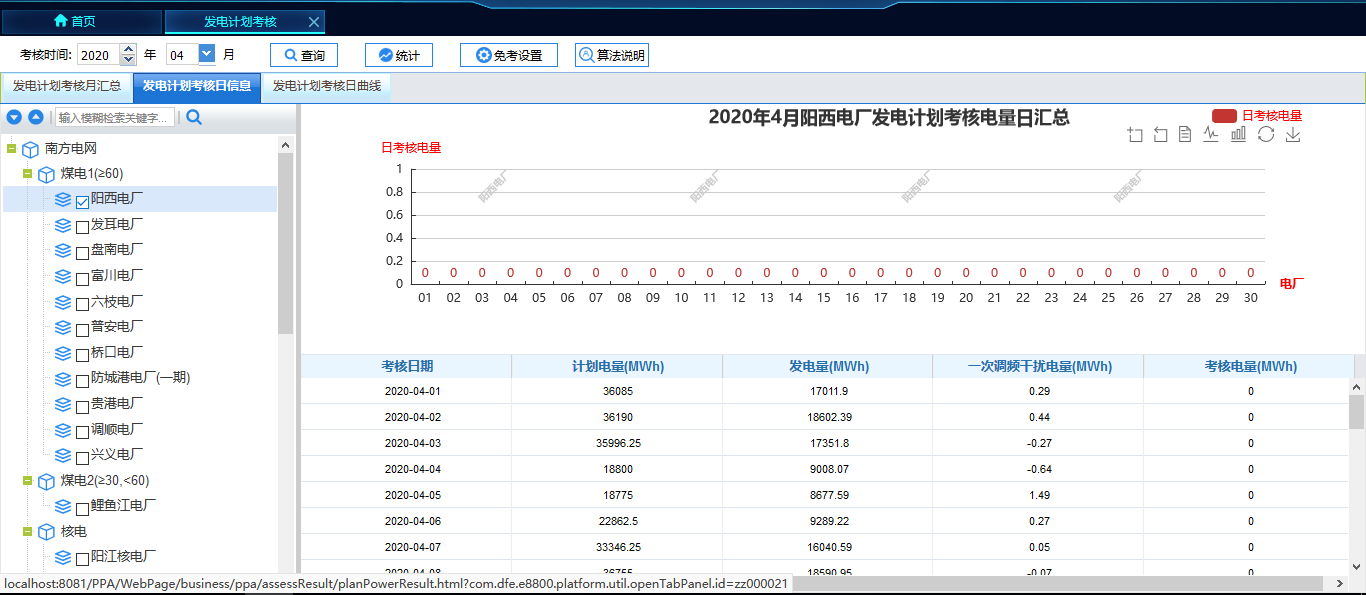
\includegraphics[width=0.7\linewidth]{pic/screenshot006}
	\caption{南方区域“两个细则”技术支持系统}
	\label{fig:screenshot006}
\end{figure}

本系统主要适用于分布式小装机容量的新能源并网机组,提供一套适用于该类机组的网——源协调分析方案,设计与分析方案相匹配的分析算法,并搭建适用于该类机组的分析平台框架。


文章第一章为绪论,主要介绍要求背景、平台开发遇到的技术难点与平台研究内容。第二章系统软件平台的实现,提出了系统软件平台的6大框架:运行环境、数据库、数据层、业务层、控制层与前端UI。第三章为一次调频考核的算法与实现,根据并网机组的特点,针对性提出了一次调频考核指标,其考核指标包括合格率和投入率两种,并对两个指标提出了相应的算法和对应的代码实现,最后使用小湾电厂2017年4月17日下午16时的数据进行了算例验算。第四章为风光预测考核的算法与实现,根据新能源发电波动性、间歇性的特点,提出了新能源功率预测考核指标,指标包括上报情况、日预测和实时预测三类,并对三种指标提出了相应的算法和对应的代码实现,最后使用三月山风电场2020年9月6日的功率数据进行算例验算。为第五章为总结与展望,总结了平台的优缺点,并对平台未来的发展做出展望。

\newpage
\section{系统软件平台}
\subsection{平台功能}
\subsubsection{概述}

电厂辅助服务分析支撑演示平台可以采集场站上传的信息,如电力系统频率,机组有功功率,机组预测功率等。平台对所采集的信息根据特定算法进行计算,并对其结果进行展示,给予调度员数据参考。

平台可以划分为两个主要部分,一是数据平台,二是考核评估平台。其中,数据平台主要收集场站上传的实测数据,包括机组实时数据、机组96点功率数据、系统频率数据等;考核评估平台主要实现详细考核数据的呈现,至今系统Demo中已实现了一次调频考核和风光预测考核两种。

\subsubsection{硬件基础}
电力系统网源协调控制系统部署一台云服务器、一台本地服务器和一台开发工作站,其中两台服务器基于Windows Server 2016平台,开发工作站基于Linux平台。

云服务器应用于应用服务器,其职能为作为平台部署发布、各模块分析计算。本地服务器用作数据库服务器,主要以MySQL储存场站上传的实时数据,完成各应用之间需要的数据储存。开发工作站主要应用于系统开发与运行维护,系统日志也储存在开发工作站中。

\subsubsection{软件平台}
基于上述的硬件平台,系统构建了运行环境、数据库、数据层、业务层、控制层与前端UI共计6大结构(如图\ref{电力系统网源协调控制系统整体结构图}所示)。
\begin{figure}[H]
	\centering
	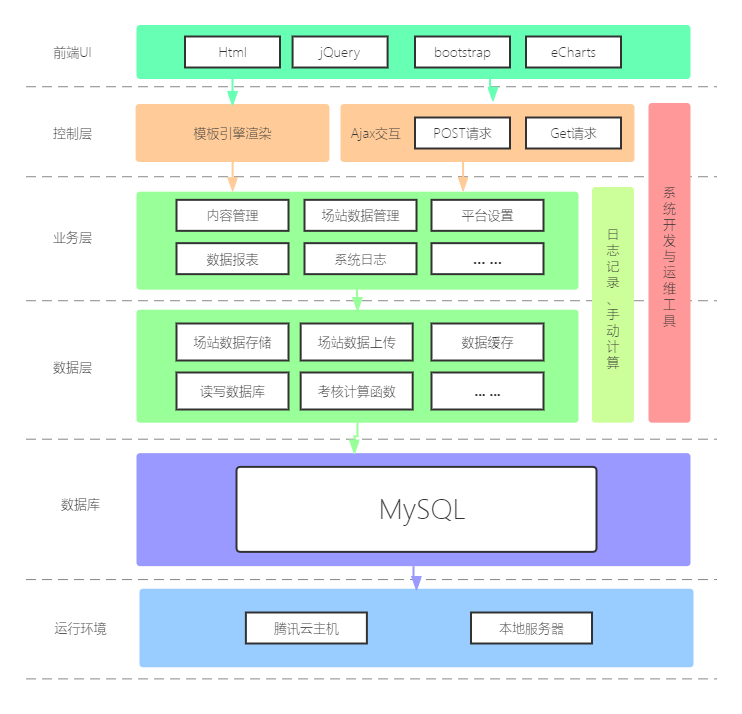
\includegraphics[width=0.9\linewidth]{pic/系统框架结构}
	\caption{电力系统网源协调控制系统整体结构图}
	\label{电力系统网源协调控制系统整体结构图}
\end{figure}

软件系统运行流程大致如下:场站侧按照系统要求对场站实际运行数据进行整理和处理,进行数据上传致数据库;数据库以特定格式储存数据后,将数据上传至应用服务器,待计算完成后将储存结果;显示终端则向应用服务器发送POST或GET请求,根据请求显示不同的数据。

\begin{figure}[H]
	\centering
	
\includegraphics[width=0.7\linewidth]{pic/软件系统示意图}
	\caption{软件系统运行流程}
	\label{软件系统运行流程}
\end{figure}
\subsection{前端UI}
\subsubsection{导航栏}
导航栏分为两部分,第一部分主要用于考核内容切换,使用Bootstrap中的导航栏类实现,其效果如图\ref{fig:screenshot026}:
\begin{figure}[H]
	\centering
	
\includegraphics[width=0.7\linewidth]{pic/screenshot026}
	\caption{导航栏}
	\label{fig:screenshot026}
\end{figure}


第二部分主要用于切换主页面与月度页面(或日板块),使用Bootstrap中的面包屑导航(Breadcrumbs)类实现:
\begin{figure}[H]
	\centering
	
\includegraphics[width=0.7\linewidth]{pic/screenshot027}
	\caption{面包屑导航(Breadcrumbs)}
	\label{fig:screenshot027}
\end{figure}

\subsubsection{主页面(年度板块)}

\paragraph{\thesubsubsection.1 代码实现}\ \\

主页面主要实现年度总览,由两个手风琴切换标签组成,分别对应考核金额和考核次数两个部分。

\begin{figure}[H]
	\centering
	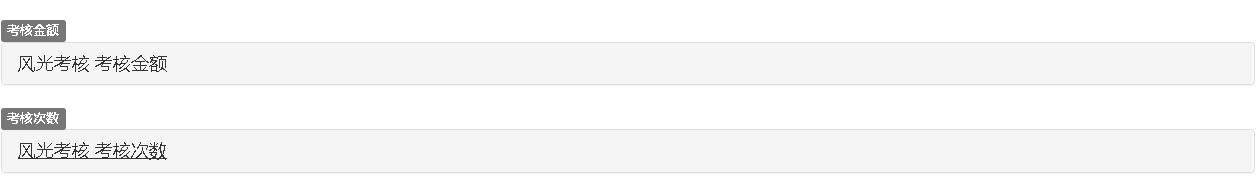
\includegraphics[width=0.7\linewidth]{pic/screenshot009}
	\caption{主页面(年度板块)的主要内容}
	\label{fig:screenshot009}
\end{figure}

其中图\ref{fig:screenshot009}中的手风琴切换样式使用Bootstrap 中的折叠(Collapse)插件实现。


折叠标签中的内容均为柱状图和表格(图\ref{fig:screenshot011}),其实现方式参考\ref{zhitu}和\ref{zhibiao}。

\begin{figure}[H]
	\centering
	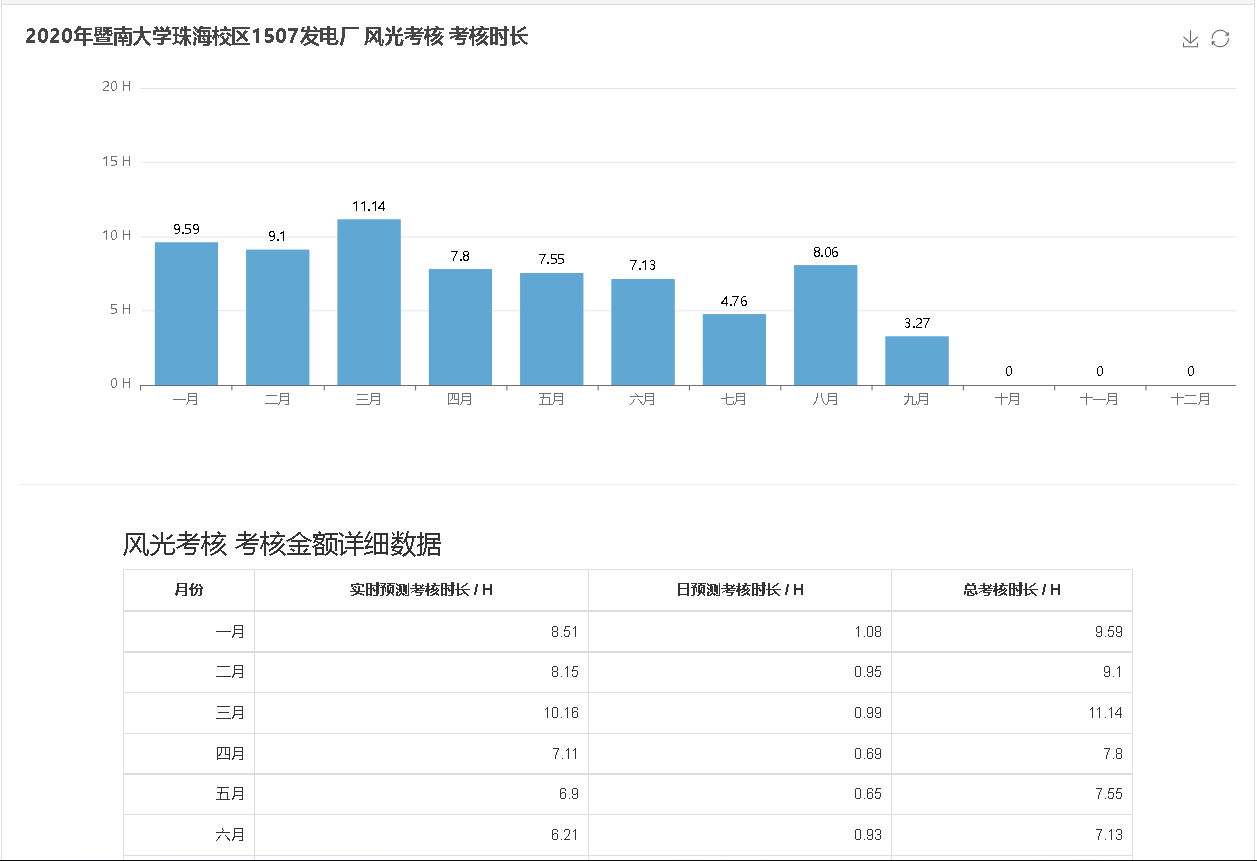
\includegraphics[width=0.7\linewidth]{pic/screenshot011}
	\caption{手风琴切换标签中的内容}
	\label{fig:screenshot011}
\end{figure}
\paragraph{\thesubsubsection.2 效果展示}\ \\

\begin{enumerate}
	\item 风光预测考核
	
	风光预测考核页面实际数据为三月山风电场2020年1-10月并网功率、短期预测功率、超短期预测功率计算,其部分结果如下:
	\begin{figure}[H]
		\centering
		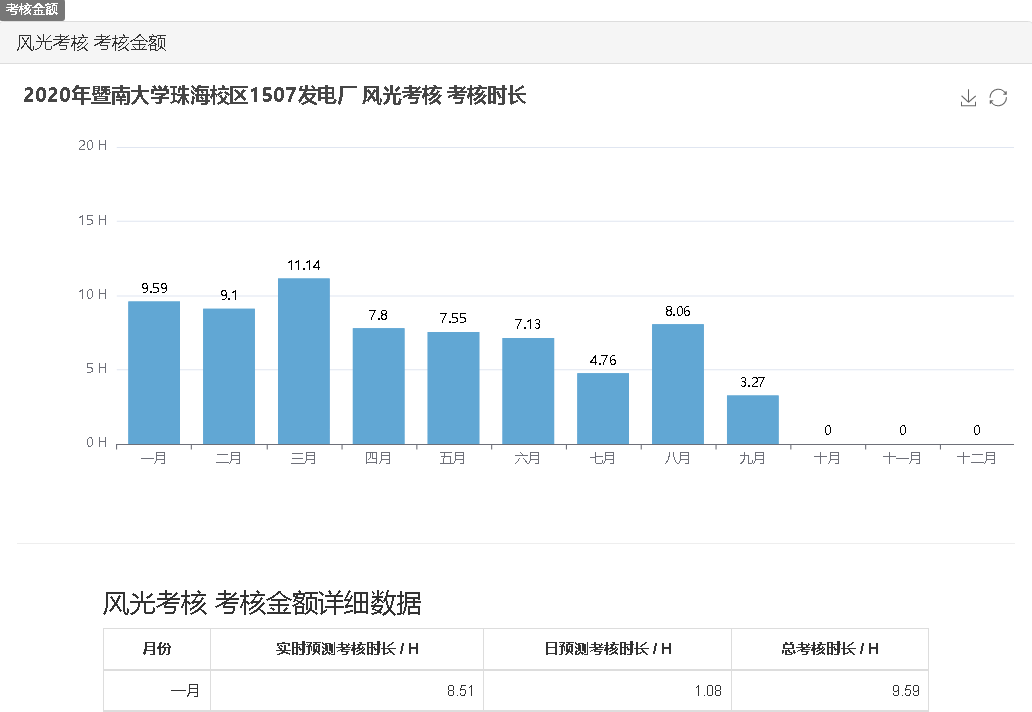
\includegraphics[width=0.7\linewidth]{pic/screenshot016_看图王}
		\caption{年度板块考核时长统计}
		\label{fig:screenshot016}
	\end{figure}
	
	%	\begin{figure}[H]
	%		\centering
	%		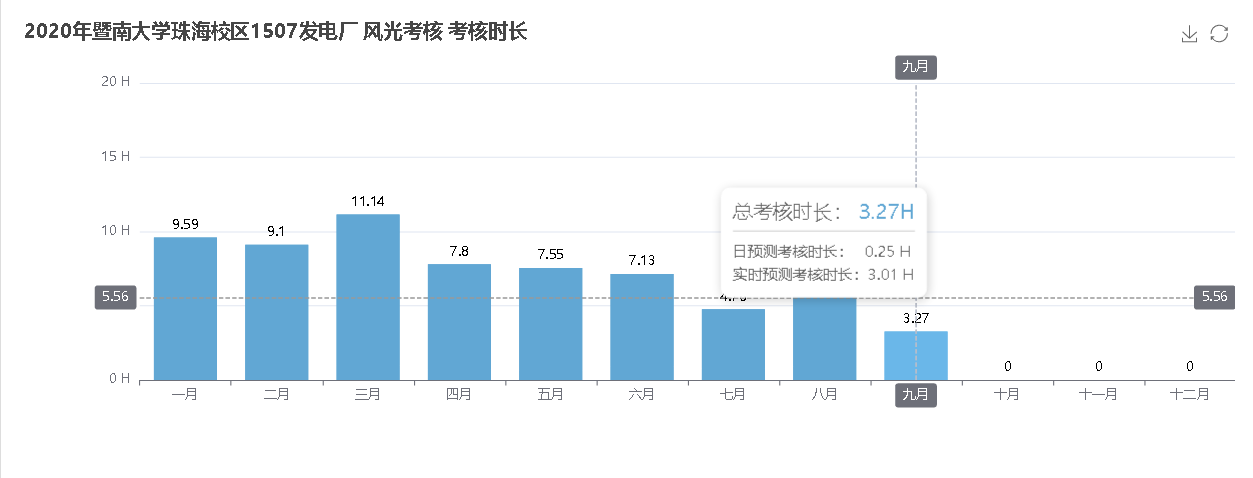
\includegraphics[width=0.7\linewidth]{pic/screenshot019}
	%		\caption{时长统计提示标签}
	%		\label{fig:screenshot019}
	%	\end{figure}
	
	\begin{figure}[H]
		\centering
		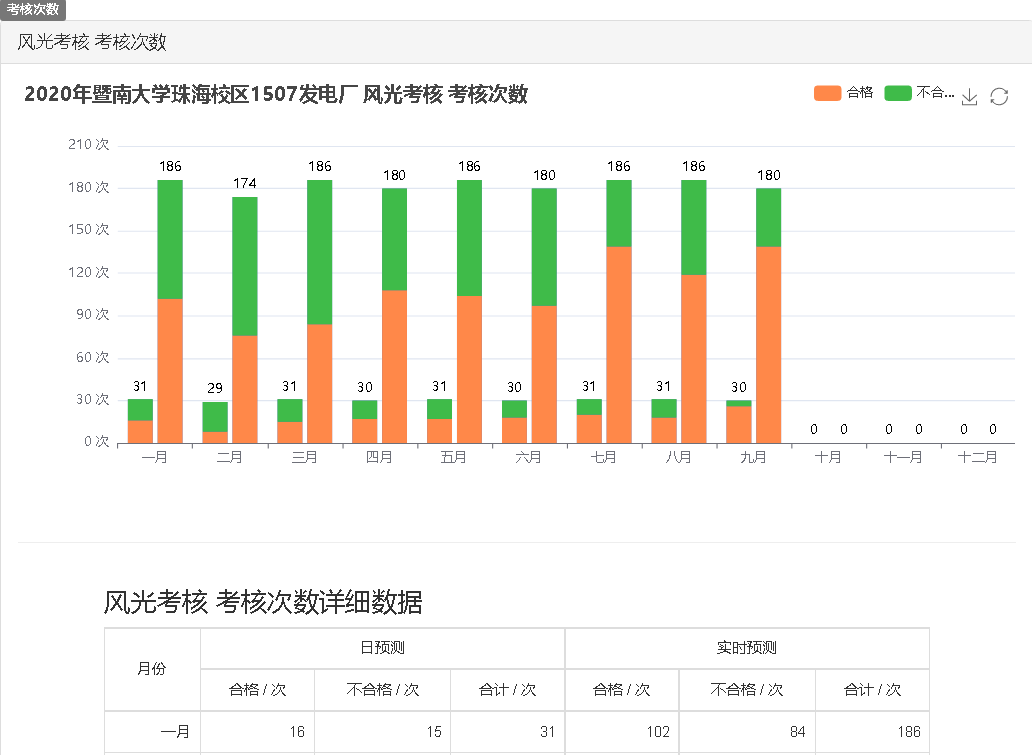
\includegraphics[width=0.7\linewidth]{pic/screenshot017_看图王}
		\caption{年度板块考核次数统计}
		\label{fig:screenshot017}
	\end{figure}
	
	%	\begin{figure}[H]
	%	\centering
	%	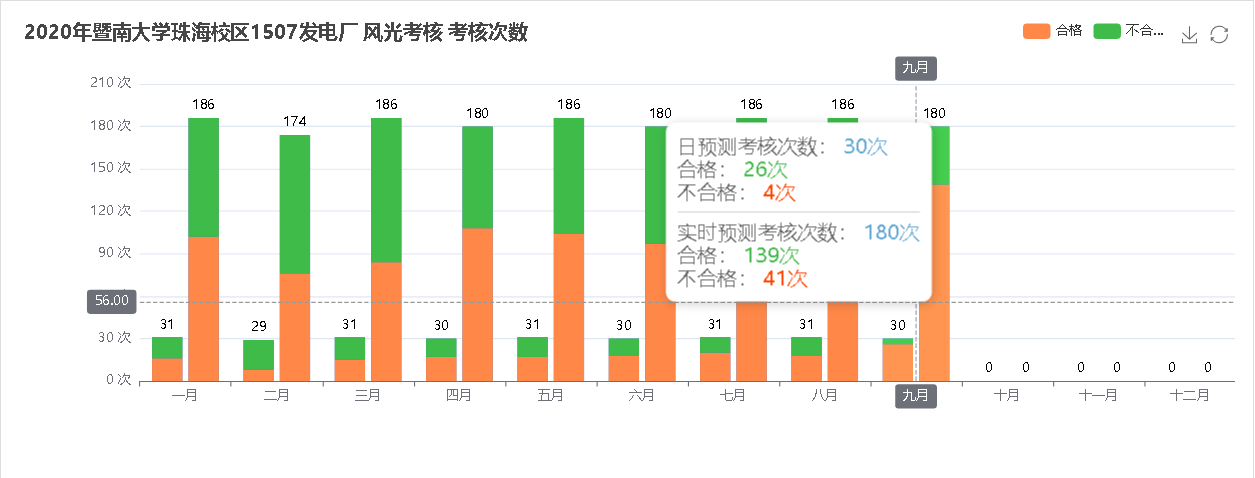
\includegraphics[width=0.7\linewidth]{pic/screenshot020}
	%	\caption{次数统计提示标签}
	%	\label{fig:screenshot020}
	%	\end{figure}
	
	\item 一次调频考核
	由于手上场站数据为残缺数据,仅有2017年4月17日下午16时到17时和2017年7月31日下午14时至15时的数据,因此一次调频考核年度页面由fakedata填充:
	\begin{figure}[H]
		\centering
		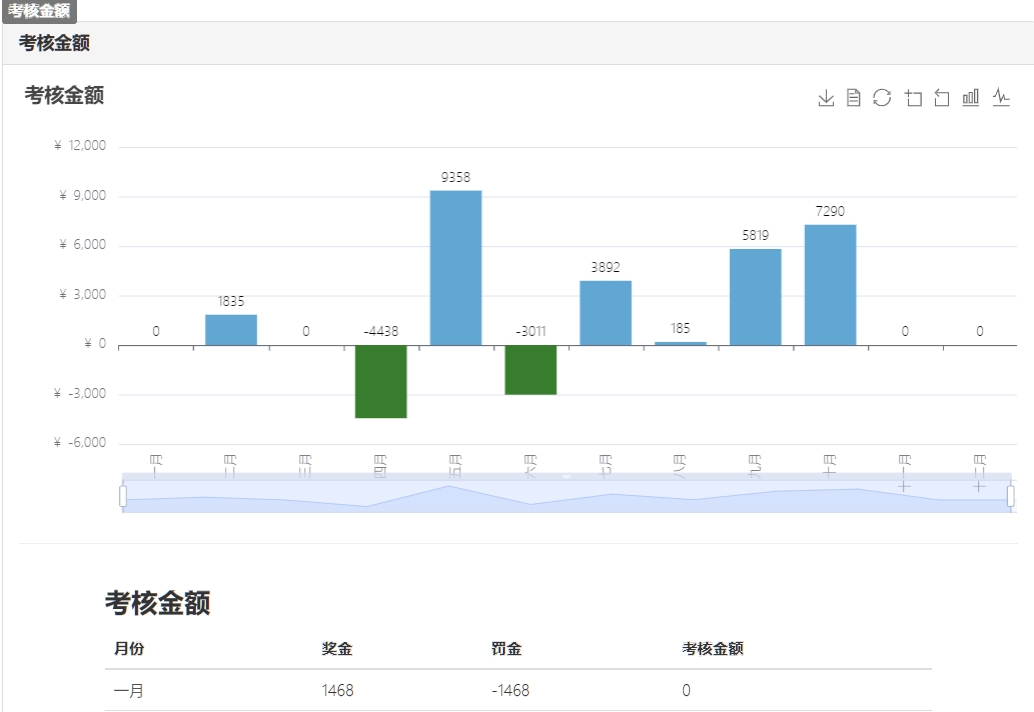
\includegraphics[width=0.7\linewidth]{pic/一次调频年度页面1}
		\caption{年度板块考核时长统计	}
		\label{fig:1}
	\end{figure}
	\begin{figure}[H]
		\centering
		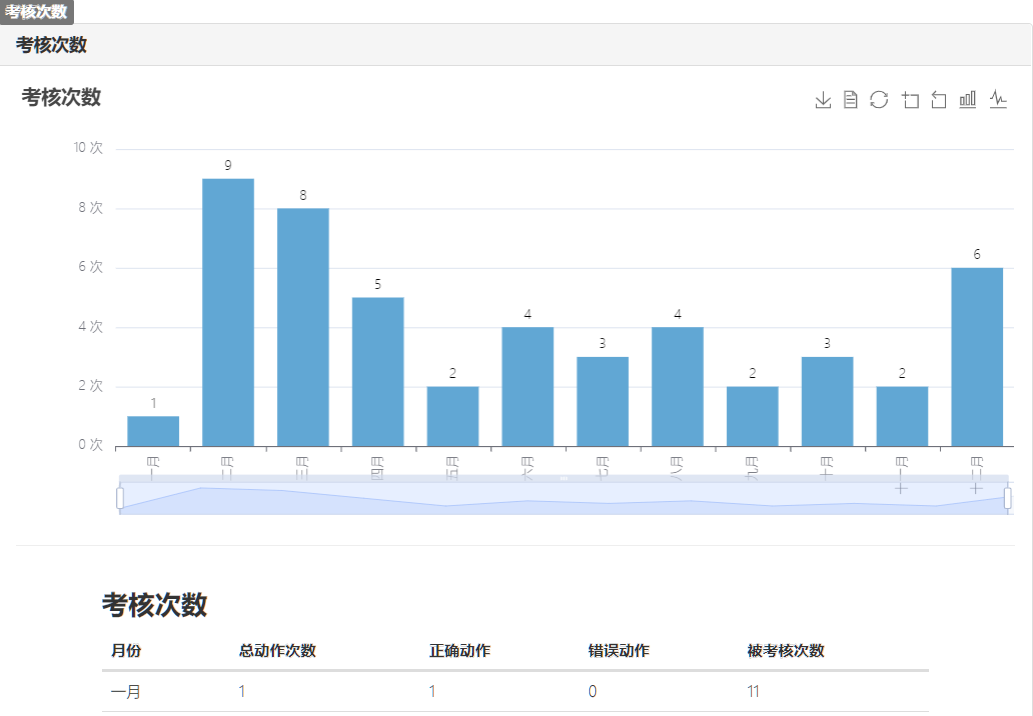
\includegraphics[width=0.7\linewidth]{pic/一次调频年度页面2}
		\caption{年度板块考核次数统}
		\label{fig:2}
	\end{figure}
	
\end{enumerate}



\subsubsection{月度板块}\label{monthbankuai}
\paragraph{\thesubsubsection.1 代码实现}\ \\
月度板块主要由数据切换模块和详细数据模块组成。
\begin{figure}[H]
	\centering
	
\includegraphics[width=0.7\linewidth]{pic/screenshot010}
	\caption{月度板块的主要内容}
	\label{fig:screenshot010}
\end{figure}

数据切换模块使用表单实现:其中不同月份选项生成主要使用封装函数“get\_dir\_files\_lists”完成,其思路为查找数据库中存在的月份数据,并使用JavaScript方法生成html标签。

\begin{figure}[H]
	\centering
	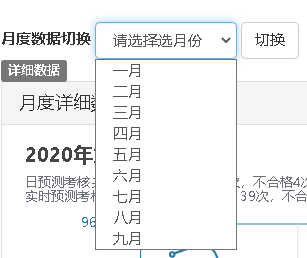
\includegraphics[width=0.3\linewidth]{pic/screenshot012}
	\caption{数据切换模块}
	\label{fig:screenshot012}
\end{figure}

手风琴切换标签内容与主页面相似。

\paragraph{\thesubsubsection.2 效果展示}\ \\
\begin{enumerate}
	\item 风光预测考核
	
	风光预测考核页面实际数据为三月山风电场2020年1-10月并网功率、短期预测功率、超短期预测功率计算,其部分结果如下:
	\begin{figure}[H]
		\centering
		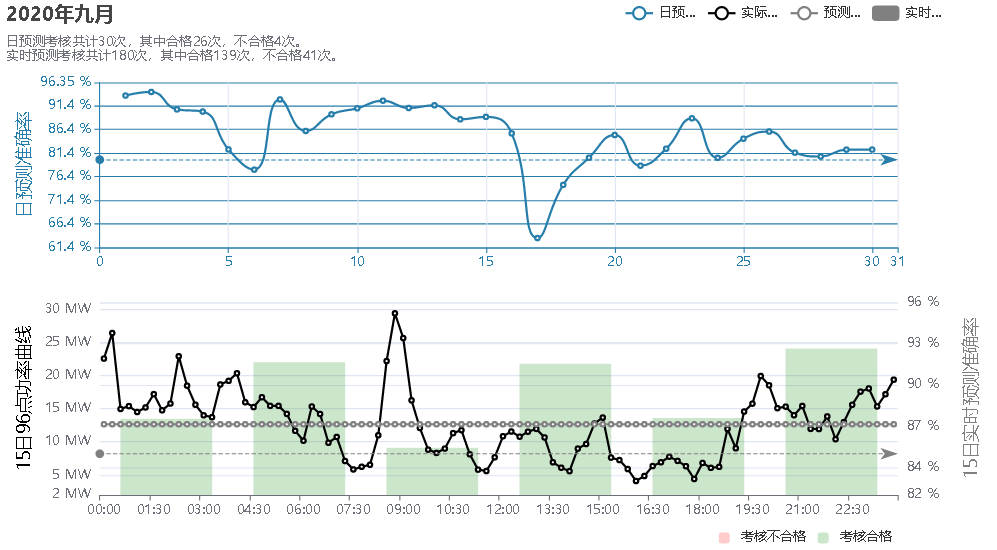
\includegraphics[width=0.7\linewidth]{pic/2020年九月}
		\caption{月度板块日预测准确率、实际功率、预测功率和实时预测准确率}
		\label{fig:2020}
	\end{figure}
	
	由于手上场站数据为残缺数据,仅有2017年4月17日下午16时到17时和2017年7月31日下午14时至15时的数据,因此一次调频考核月度页面由fakedata填充:
	\begin{figure}[H]
		\centering
		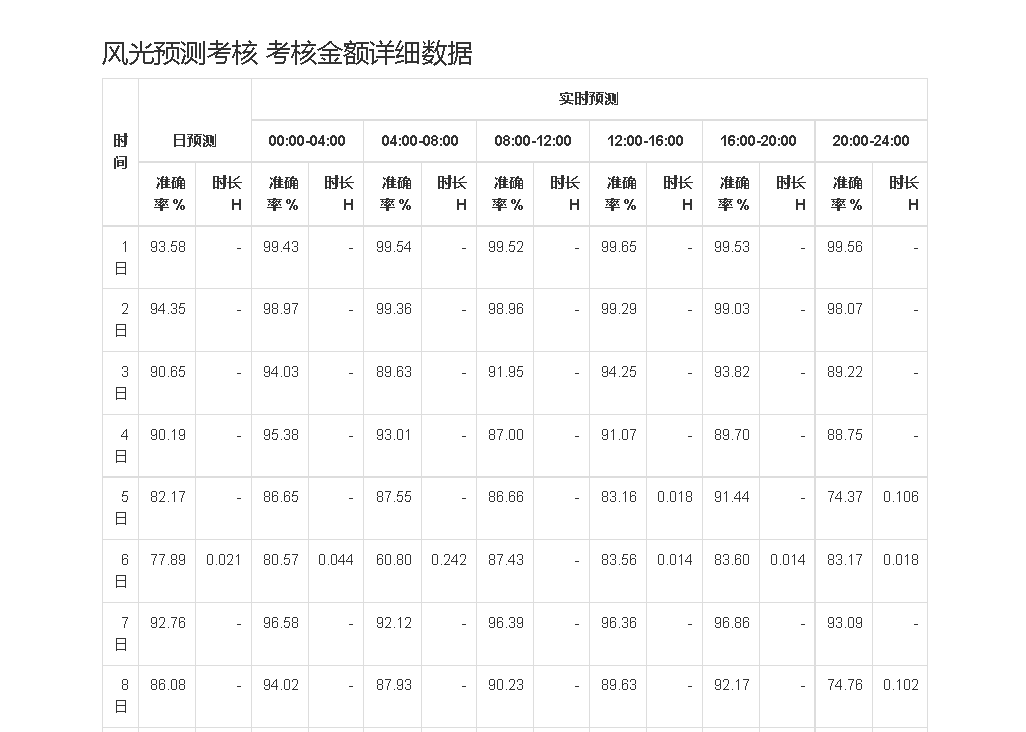
\includegraphics[width=0.7\linewidth]{pic/screenshot021}
		\caption{月度板块考核详细数据表格}
		\label{fig:screenshot021}
	\end{figure}
	\item 一次调频考核
	
	
	\begin{figure}[H]
		\centering
		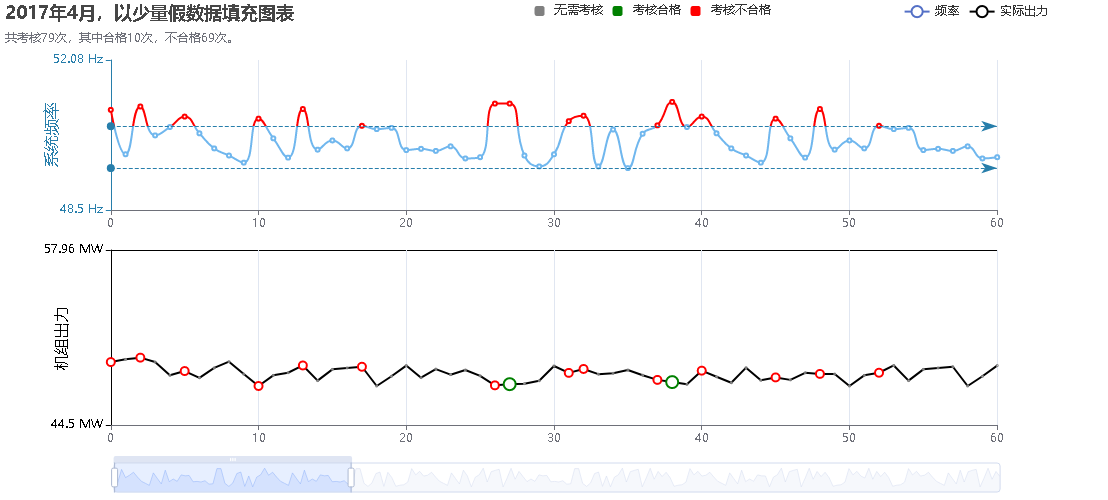
\includegraphics[width=0.7\linewidth]{pic/2017年4月,以少量假数据填充图表}
		\caption{月度板块频率,实际功率和考核情况}
		\label{fig:20174}
	\end{figure}
	\begin{figure}[H]
		\centering
		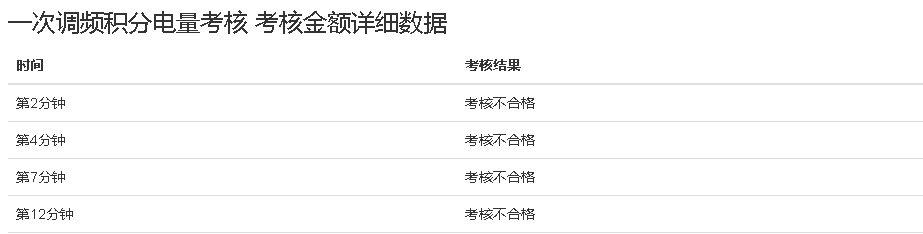
\includegraphics[width=0.7\linewidth]{pic/screenshot023}
		\caption{月度板块考核详细数据表格}
		\label{fig:screenshot023}
	\end{figure}
\end{enumerate}
\subsubsection{日板块}
\paragraph{\thesubsubsection.1 代码实现}\ \\
日板块仅对一次调频考核生效,其实现与\ref{monthbankuai}相同,不同之处仅为所传入的数据。
\paragraph{\thesubsubsection.2 效果展示}\ \\

日板块使用2017年4月17日下午16时到17时小湾水电站的有功功率、频率进行计算,其结果呈现如下:
\begin{figure}[H]
	\centering
	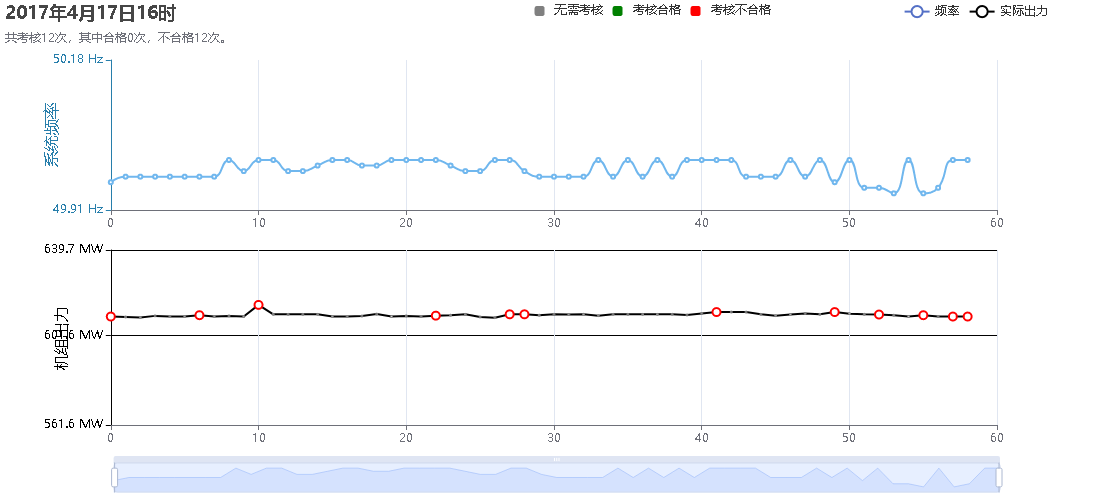
\includegraphics[width=0.7\linewidth]{pic/2017年4月17日16时}
	\caption{小湾水电站2017年4月17日16时日考核}
	\label{fig:201741716}
\end{figure}
\subsection{控制层}
\subsubsection{制图}\label{zhitu}


ECharts是基于zrender的高级封装\upcite{li2018echarts},是百度旗下的产品。其开源、免费、易用的特性使得许多可视化产品都使用该库进行。本文的制图工具选用echarts进行。

ECharts脚本使用json进行配置,配置方式较为简单,下面简要说明一下一些主要配置:
\paragraph{\thesubsubsection.1 dataset}\ \\

dataset是echarts的数据集传入方式之一,可以方便地被多个系列复用,并且在后续的tooltip提示框中更为方便地调用,因此本文中主要以这种形式传递数据。

一般而言,数据一般都可以储存为广义的二维数组,即每一个点中需要的全部数据可以记为一个一维数组,因此,整个数据集可以看作一个包含每一个点的二维数组。echarts中dataset即为这种思维。在dataset中,一般需要指定dimensions和source。dimensions可以简单理解为字典中的key,source则为对应的value,在后续中便可以根据指定的dimensions进行配置需要的作图数据。

\textit{附录B-系统功能软件平台-控制层-dataset数据初始化}中的代码为风电数据的dataset初始化示例。


\paragraph{\thesubsubsection.2 series}\label{xAxisIndexyAxisIndex}\ \\

series为作图系列。每一个图都对应为一个series。这里主要用折线图和柱状图,对应的为series.line和series.bar。


当需要绘制多个图时,需要指定x、y坐标的位置。如图\ref{fig:screenshot002}中日预报准确率的参数,设置参数为:	xAxisIndex: 0,yAxisIndex: 0,gridIndex: 0,其表示使用第一个x轴,第一个y轴和第一个图表位置。
\begin{figure}[H]
	\centering
	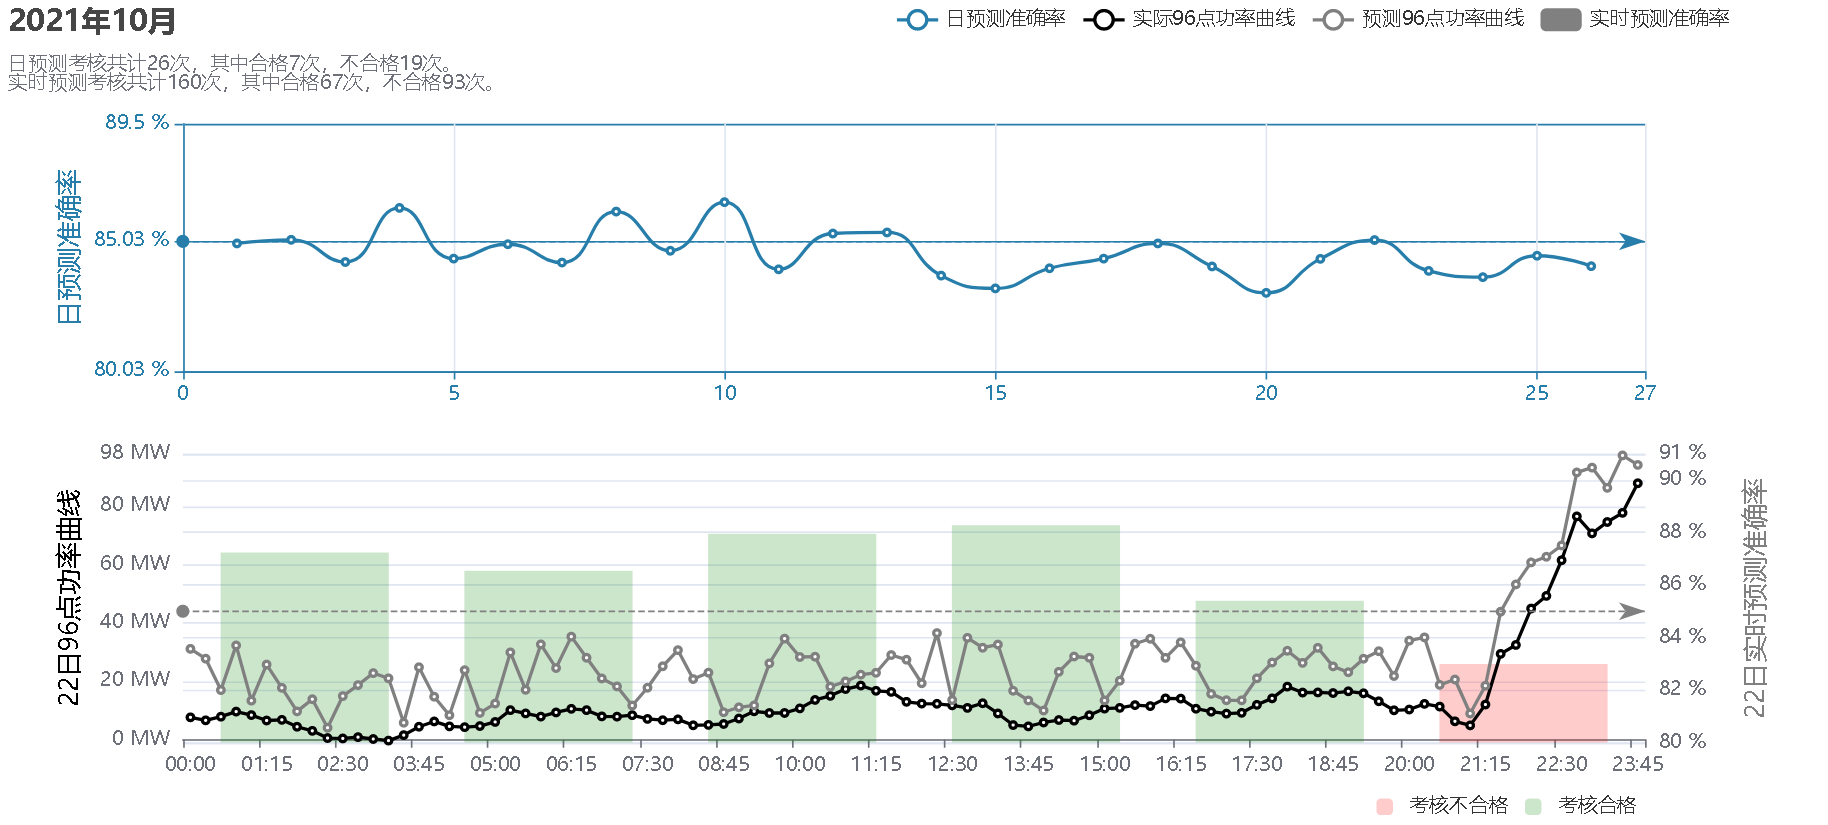
\includegraphics[width=0.8\linewidth]{pic/screenshot002}
	\caption{多个图表实例}
	\label{fig:screenshot002}
\end{figure}
在series中使用encode即可指定作图用的dimensions,从而自由地使用dataset中的指定数据。使用风电预测考核作为例子,其encode的代码见\textit{附录B-系统功能软件平台-控制层-使用encode选择数据}。


\paragraph{\thesubsubsection.3 visualmap}\ \\

visualmap是echarts的视觉映射组件,虽然其功能可以在series.color中使用自定义函数实现,但是使用visualmap封装则可以简化程序。
\begin{figure}[H]
	\centering
	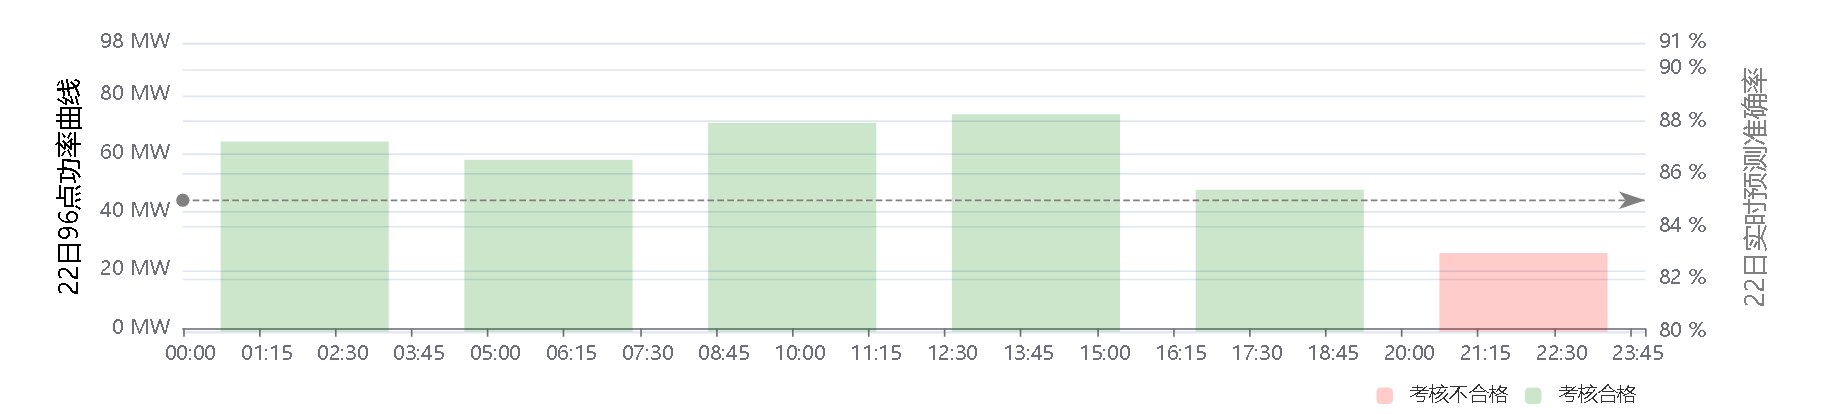
\includegraphics[width=0.8\linewidth]{pic/screenshot003}
	\caption{visualmap示例}
	\label{fig:screenshot003}
\end{figure}

visualmap分为两种,连续型continuous和分段型piecewise。本文中一般使用分段型piecewise。图\ref{fig:screenshot003}的例子是使用\textit{附录B-系统功能软件平台-控制层-对visualmap进行配置}中的代码进行配置的。




\paragraph{\thesubsubsection.4 tooltip}\ \\

tooltip是提示框组件,其可选择放置于全局或者仅作用于某一系列。本文中使用全局配置。

\begin{figure}[H]
	\centering
	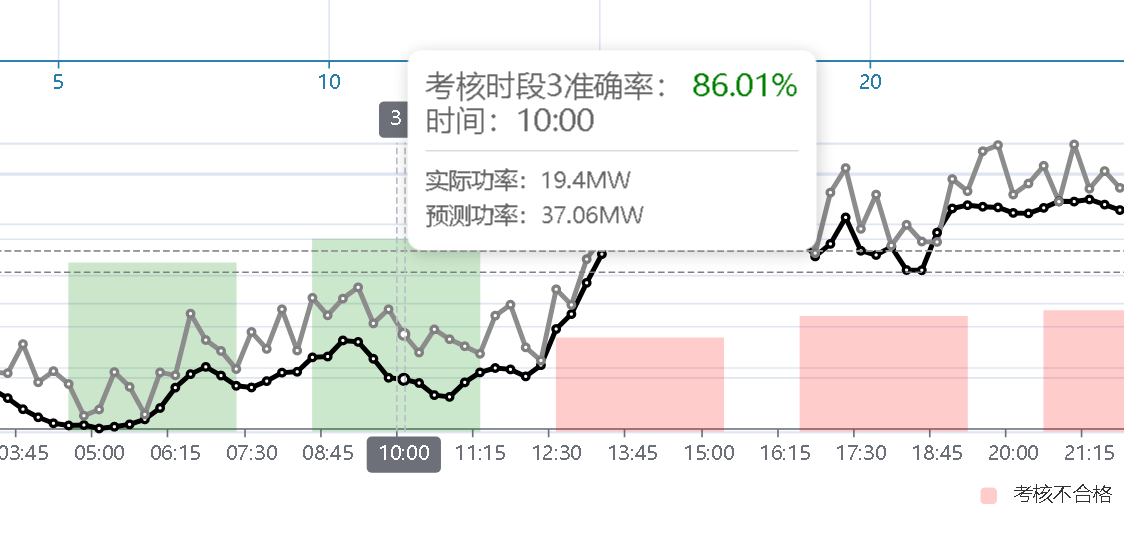
\includegraphics[width=0.8\linewidth]{pic/screenshot001}
	\caption{tooltip提示框}
	\label{fig:screenshot001}
\end{figure}

tooltip是作为交互式体验的重要部分,当tooltip触发的时候,可以根据触发时传入的数据进行一定的配置,从而实现数据可视化交互。如图\ref{fig:screenshot001}所示,可以直观看到当前鼠标所指的系列的详细数据。

tooltip常用的配置参数有
\begin{enumerate}
	\item trigger 触发位置
	
	一般选用 Axis,即坐标轴触发
	\item axisPointer 指针位置提示
	\item showDelay 显示延迟
	\item hideDelay 隐藏延时
	\item position 提示框出现位置
	
	默认情况下,提示框会出现在鼠标右方,因此在某系情况下会有遮挡的问题。此时需要对出现位置进行修正,其过程如图\ref{提示框位置}所示:
	
	\begin{figure}[H]  
		\centering
		\scriptsize  
		\begin{tikzpicture}[node distance=2cm,]
			\node (start) [startstop] {鼠标位置修正};
			\node (in1) [io, below of=start, xshift=-3cm] {鼠标位置参数};
			\node (in2) [io, right of=in1, xshift=4cm] {图像窗格大小参数};
			
			\node (dec1) [decision, below of=in1, yshift=-1cm,xshift=3cm, align=center] {鼠标在图\\像左半边};
			\node (stop1) [startstop, left of=dec1, align=center,xshift=-2cm] {提示框左下角\\为鼠标指针位置};
			\node (stop2) [startstop, right of=dec1, align=center,xshift=2cm] {提示框右下角\\为鼠标指针位置};
			%				\node (stop1) [startstop, below of=dec1,,yshift=-1cm] {无需考核};
			%				\node (stop2) [startstop, below of=dec2,,yshift=-1cm] {考核不合格};
			%				\node (stop3) [startstop, right of=dec2,,xshift=1.5cm] {考核合格};
			%连接具体形状
			\draw [arrow](start) -- (in1);
			\draw [arrow](start) -- (in2);
			%				\draw[arrow] (
			%				in1.west)-- node[] {} ($(in1.west) - (1.05,0)$) |- ($(dec1.west)-(0.8,0)$) -- (dec1.west);
			\draw [arrow](in1.south) -- (dec1.north);
			\draw [arrow](in2.south) -- (dec1.north);
			%				\draw [arrow](pro1.south) -- (dec2.west);
			%				\draw [arrow](pro2) -- (dec2);
			%				\draw [arrow](dec2) -- node[anchor=east,above=0.5mm] {否} (stop3);
			%				\draw [arrow](dec2) -- node[anchor=south,above=-1mm,left=0.5mm] {是} (stop2);
			\draw [arrow](dec1) -- node[anchor=east,above=1mm] {是} (stop1);
			\draw [arrow](dec1) -- node[anchor=west,above=1mm] {否} (stop2);
			
			
		\end{tikzpicture}
		\caption{提示框位置计算流程图}
		\label{提示框位置}
	\end{figure}  
	
	使用该方法即可使得提示框出现位置为鼠标左上方,即可解决遮挡现象。其实现代码见\textit{附录B-系统功能软件平台-控制层-鼠标位置修正}。
	\item formatter 提示框中字符格式
	
	默认情况下,提示框提示仅有绘图数据。但本文中需要的并不仅仅只有绘图中的数据,还有其背后的考核时间等不在图中显示的数据,此时便需要使用formatter进行自定义。formatter可以使用HTML文本传输,图\ref{fig:screenshot001}中使用\textit{附录B-系统功能软件平台-控制层-提示框字符格式}中的代码生成。
	
	
	
\end{enumerate}
\paragraph{\thesubsubsection.5 toolbox}\ \\

toolbox为工具箱,内置有导出图片,数据视图,动态类型切换,数据区域缩放,重置五个工具。本文中取用导出图片与重置工具。
\begin{figure}[H]
	\centering
	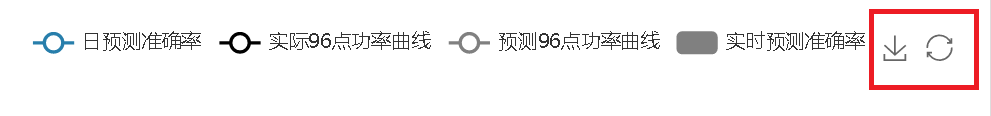
\includegraphics[width=0.7\linewidth]{pic/screenshot004}
	\caption{左:导出图片;右:重置}
	\label{fig:screenshot004}
\end{figure}


\paragraph{\thesubsubsection.6 grid}\label{grid}\ \\

grid是建立不同的绘图区域,在其中可以定义图片宽度、高度和位置。当绘图时,仅需在series中指定gridIndex即可完成切换。如图\ref{fig:screenshot002},上下两个绘图区域配置的代码详见\textit{附录B-系统功能软件平台-控制层-grid设置}。



\paragraph{\thesubsubsection.7 xAxis和yAxis}\ \\

xAxis和yAxis分别是x方向和y方向的坐标轴。和\ref{grid}中grid一样,xAxis和yAxis可以建立多个x或y轴,在series中如\ref{xAxisIndexyAxisIndex}中第一段代码设置即可指定所使用的坐标轴。

\paragraph{\thesubsubsection.8 自动缩放}\ \\

在实际浏览中,由于使用者的设备屏幕大小不一定相同,因此若使用固定绘图区域大小则可能出现图片过大或过小的问题。其实现过程如图\ref{自动缩放}:
\begin{figure}[H]  
	\centering
	\scriptsize  
	\begin{tikzpicture}[node distance=2cm,]
		\node (start) [startstop] {自动缩放};
		\node (in1) [io, below of=start,] {图像窗格大小};
		\node (in2) [io, below of=in1, ] {页面大小};
		
		\node (dec1) [decision, below of=in2, yshift=-1cm, align=center] {页面大小\\是否变动};
		\node (stop1) [startstop, left of=dec1, align=center,xshift=-2cm] {根据新页面大小\\重设图像窗格大小};
		
		%				\node (stop1) [startstop, below of=dec1,,yshift=-1cm] {无需考核};
		%				\node (stop2) [startstop, below of=dec2,,yshift=-1cm] {考核不合格};
		%				\node (stop3) [startstop, right of=dec2,,xshift=1.5cm] {考核合格};
		%连接具体形状
		\draw [arrow](start) -- (in1);
		\draw [arrow](in1) -- (in2);
		%				\draw[arrow] (
		%				in1.west)-- node[] {} ($(in1.west) - (1.05,0)$) |- ($(dec1.west)-(0.8,0)$) -- (dec1.west);
		%			\draw [arrow](in1.south) -- (dec1.north);
		\draw [arrow](in2.south) -- (dec1.north);
		%				\draw [arrow](pro1.south) -- (dec2.west);
		%				\draw [arrow](pro2) -- (dec2);
		%				\draw [arrow](dec2) -- node[anchor=east,above=0.5mm] {否} (stop3);
		%				\draw [arrow](dec2) -- node[anchor=south,above=-1mm,left=0.5mm] {是} (stop2);
		\draw [arrow](dec1) -- node[anchor=east,above=1mm] {是} (stop1);
		\draw [arrow](dec1.east) |- node[anchor=east,above=1mm]{否}($(dec1.east) + (1.05,0)$) |- ($(in1.north)+(0.8,0.5)$) |- ($(in1.north)+(0,0.5)$);
		\draw [arrow](stop1.north) |- node[]{} ($(in1.north)-(1,-0.7)$) |- ($(in1.north)+(0,0.7)$);
		
	\end{tikzpicture}
	\caption{自动缩放流程图}
	\label{自动缩放}
\end{figure} 

echarts中对此过程进行里封装,在实际编程中可以使用\textit{附录B-系统功能软件平台-控制层-自动缩放}中的代码对图表进行自动缩放。

\paragraph{\thesubsubsection.9 动态绘制}\ \\

在本系统中,绘图的数据其实并非一成不变的,而是动态变化的。由于echarts使用json进行绘图配置,因此很容易便可实现动态图表的绘制,过程如图 \ref{dthz}:

\begin{figure}[H]  
	\centering
	
	\scriptsize  
	
	%像素点,用于连接转移线
	\begin{tikzpicture}[node distance=2cm]
		%定义流程图具体形状
		\node (start1) [startstop] {动态绘制};
		\node (in1) [io, below of=start1] {获取新绘制数据};
		\node (pro1) [process, below of=in1,] {更改绘图配置};
		\node (pro2) [process, below of=pro1] {传入绘图配置};
		\node (stop1) [startstop, below of=pro2]{重新渲染};
		
		%连接具体形状
		\draw [arrow](start1) -- (in1);
		\draw [arrow](in1) --  (pro1);
		\draw [arrow](pro1) -- (pro2);
		\draw [arrow](pro2) --  (stop1);
		
	\end{tikzpicture}
	\caption{动态绘制流程图}
	\label{dthz}
\end{figure} 

下面以风电预测的阅读详情页面进行简单说明:

在echarts中封装了截获鼠标操作状态的函数,只需要向其传入相应的鼠标代码即可触发,可选参数有'click'、'mousedown'、'mousemove'等。当鼠标发送鼠标单击命令时,即触发function中的行为。此时,仅需要在function对绘图配置进行修改,即可实现动态绘图。\textit{附录B-系统功能软件平台-控制层-动态绘制}中的代码可以实现对图\ref{fig:screenshot002}的动态重绘。

\subsubsection{表格生成}\label{zhibiao}
在绘图脚本中,我们使用了ECharts。其实在ECharts库中有显示绘制数据的函数,可以在options中使用toolbox语句调用。

但表格呈现的内容并不仅仅有图片上的信息,还有图片上不能呈现的信息,如动作正确次数,动作错误次数,动作时间等。这些信息就需要使用额外表格进行呈现。

在html中,表格使用<table></table>进行初始化,<thead></thead>表示表头,<td></td>表示行,<tr></tr>表示列。如果把表格看做一个二维数组,那么每一个行与列都对应一个特定的坐标,因此实际编程中,可以先生成行,再生成列,然后根据其当前坐标向列中填充具体的数据。据此,可以整理出表格绘制的流程(图\ref{表格绘制}):
\begin{figure}[H]  
	\centering
	\scriptsize  
	\begin{tikzpicture}[node distance=2cm,]
		\node (start) [startstop] {表格绘制};
		\node (in1) [io, below of=start,] {表格数据(二维数组)};
		\node (pro1) [process, below of=in1, ] {生成行};
		\node (pro2) [process, below of=pro1, ] {生成列};
		\node (dec1) [decision, below of=pro2,yshift=-0.5cm, align=center] {当前列\\已完成};
		\node (dec2) [decision, below of=dec1,yshift=-2cm, align=center] {当前行\\已完成};
		\node (stop1) [startstop, below of=dec2,yshift=-0.5cm, align=center] {表格绘制完成};
		\draw [arrow](start) -- (in1);
		\draw [arrow](in1) -- (pro1);
		\draw [arrow](pro1) -- (pro2);
		\draw [arrow](pro2) -- (dec1);
		\draw [arrow](dec1) -- node[anchor=south,left=1mm] {是}(dec2);
		\draw [arrow](dec2) -- node[anchor=south,left=1mm] {是}(stop1);
		\draw [arrow](dec1.east) -- node[anchor=east,above=1mm]{否}($(dec1.east) + (1.05,0)$) |- ($(pro2.north)+(1.6,0.5)$) |- ($(pro2.north)+(0,0.5)$);
		\draw [arrow](dec2.west) -- node[anchor=west,above=1mm]{否}($(dec2.west) - (1.05,0)$) |- ($(pro1.north)-(1.6,-0.5)$) |- ($(pro1.north)+(0,0.5)$);
		
	\end{tikzpicture}
	\caption{表格绘制流程图}
	\label{表格绘制}
\end{figure} 

此处把脚本封装为JavaScript函数,其代码见\textit{附录B-系统功能软件平台-控制层-表格绘制}。调用该函数即可进行表格绘制。

\subsection{业务层}
\subsubsection{考核结果运算}
在\ref{uploadfile}中,我们定义了文件上传使用“年-月”的规则进行储存数据,若需要重新计算全部考核结果,则可以通过遍历年数据库,然后在年数据库中遍历月数据库,再根据月数据运算考核结果。因此可以用如图\ref{考核结果运算}的流程进行考核结果运算:
\begin{figure}[H]  
	\centering
	\scriptsize  
	\begin{tikzpicture}[node distance=2cm,]
		\node (start) [startstop] {考核结果运算};
		\node (in1) [io, below of=start,] {数据库数据};
		\node (pro1) [process, below of=in1, ] {进入年数据库};
		\node (pro2) [process, below of=pro1, ] {进入月数据库};
		\node (pro3) [process, below of=pro2, ] {运算考核结果};
		\node (dec1) [decision, below of=pro3,yshift=-0.5cm, align=center] {当前月\\已完成};
		\node (dec2) [decision, below of=dec1,yshift=-2cm, align=center] {当前年\\已完成};
		\node (stop1) [startstop, below of=dec2,yshift=-0.5cm, align=center] {考核结果运算完成};
		\draw [arrow](start) -- (in1);
		\draw [arrow](in1) -- (pro1);
		\draw [arrow](pro1) -- (pro2);
		\draw [arrow](pro2) -- (pro3);
		\draw [arrow](pro3) -- (dec1);
		\draw [arrow](dec1) -- node[anchor=south,left=1mm] {是}(dec2);
		\draw [arrow](dec2) -- node[anchor=south,left=1mm] {是}(stop1);
		\draw [arrow](dec1.east) -- node[anchor=east,above=1mm]{否}($(dec1.east) + (1.05,0)$) |- ($(pro2.north)+(1.6,0.5)$) |- ($(pro2.north)+(0,0.5)$);
		\draw [arrow](dec2.west) -- node[anchor=west,above=1mm]{否}($(dec2.west) - (1.05,0)$) |- ($(pro1.north)-(1.6,-0.5)$) |- ($(pro1.north)+(0,0.5)$);
	\end{tikzpicture}
	\caption{考核结果运算流程图}
	\label{考核结果运算}
\end{figure} 

将上述流程封装为php函数,其代码见\textit{附录B-系统功能软件平台-业务层-考核结果运算}。封装函数其中\$y,\$m分别为年和月,传入相应的参数即可实现计算考核结果。


\subsection{数据层}
\subsubsection{文件上传页面的实现}\label{uploadfile}
\begin{figure}[H]
	\centering
	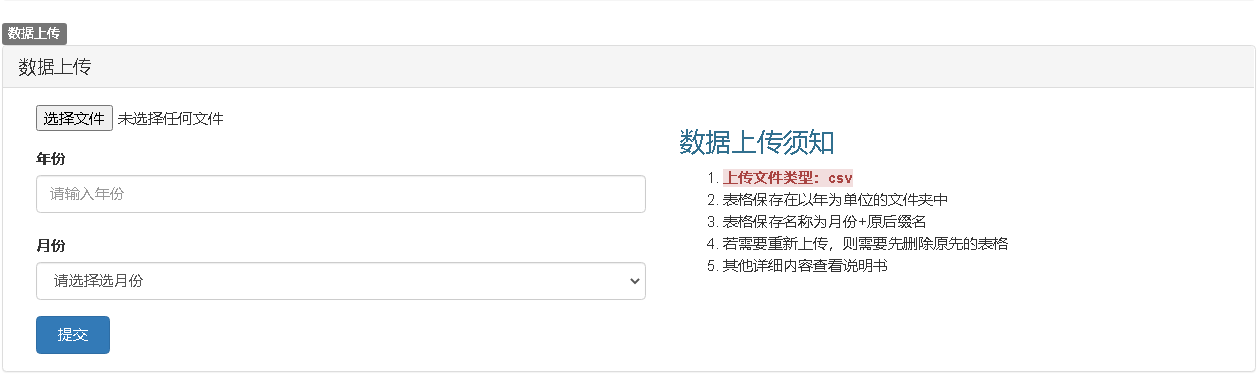
\includegraphics[width=0.7\linewidth]{pic/screenshot013}
	\caption{数据切换模块}
	\label{fig:screenshot013}
\end{figure}


文件上传页面主要实现文件上传与储存功能,主要使用HTMl中的文件上传表单配合PHP实现。文件上传页面的html前端代码见\textit{附录B-系统功能软件平台-数据层-文件上传页面}。


\subsubsection{异常处理}

在文件上传过程中,若不符合上传规定,则应提示用户重新选择参数。

\paragraph{\thesubsubsection.1 文件格式错误}\label{fileerror}\ \\

文件上传要求格式为csv格式,若选择的文件为其他类型,则终止上传过程并提示用户:
\begin{figure}[H]
	\centering
	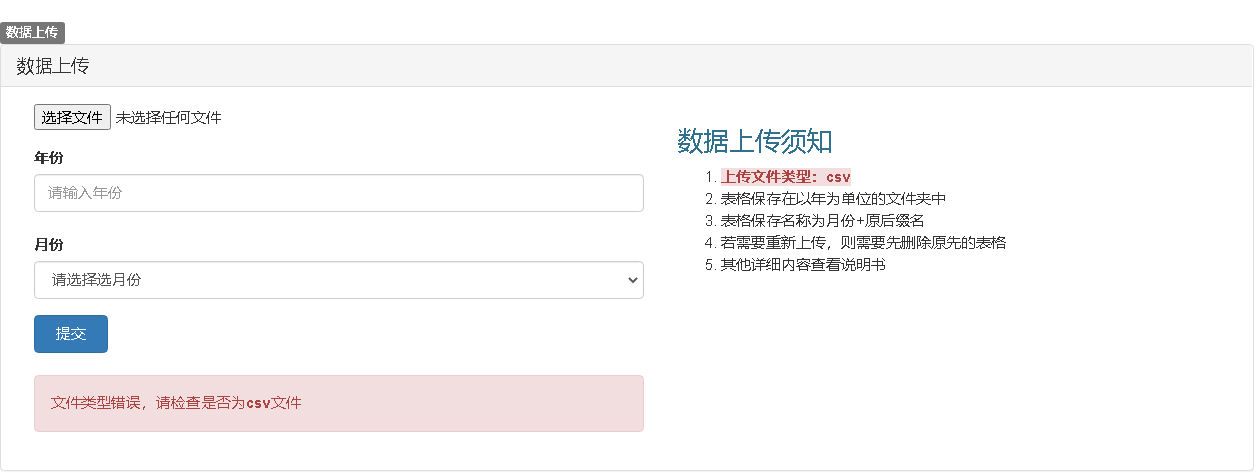
\includegraphics[width=0.7\linewidth]{pic/screenshot014}
	\caption{文件格式错误}
	\label{fig:screenshot014}
\end{figure}

格式错误提示整体流程如图\ref{文件格式校验},其php代码如\textit{附录B-系统功能软件平台-数据层-文件格式错误}所示。
\begin{figure}[H]  
	\centering
	\scriptsize  
	\begin{tikzpicture}[node distance=2cm,]
		\node (start) [startstop] {文件格式校验};
		\node (in1) [io, below of=start,] {传入文件};
		\node (dec1) [decision, below of=in1,yshift=-0.5cm, align=center] {文件格式\\为csv};
		\node (stop2) [startstop, left of=dec1,xshift=-2cm, align=center] {显示文件\\式错误,终止上传};
		\node (stop1) [startstop, right of=dec1,xshift=2cm, align=center] {无需提示,\\文件正常上传};
		\draw [arrow](start) -- (in1);
		\draw [arrow](in1) -- (dec1);
		\draw [arrow](dec1) -- node[anchor=south,above=1mm] {是}(stop1);
		\draw [arrow](dec1) -- node[anchor=south,above=1mm] {否}(stop2);
	\end{tikzpicture}
	\caption{文件格式校验流程图}
	\label{文件格式校验}
\end{figure} 


\paragraph{\thesubsubsection.2 未选择年份或月份}\ \\

若用户未选择年份或月份,则终止上传过程并提示用户:
\begin{figure}[H]
	\centering
	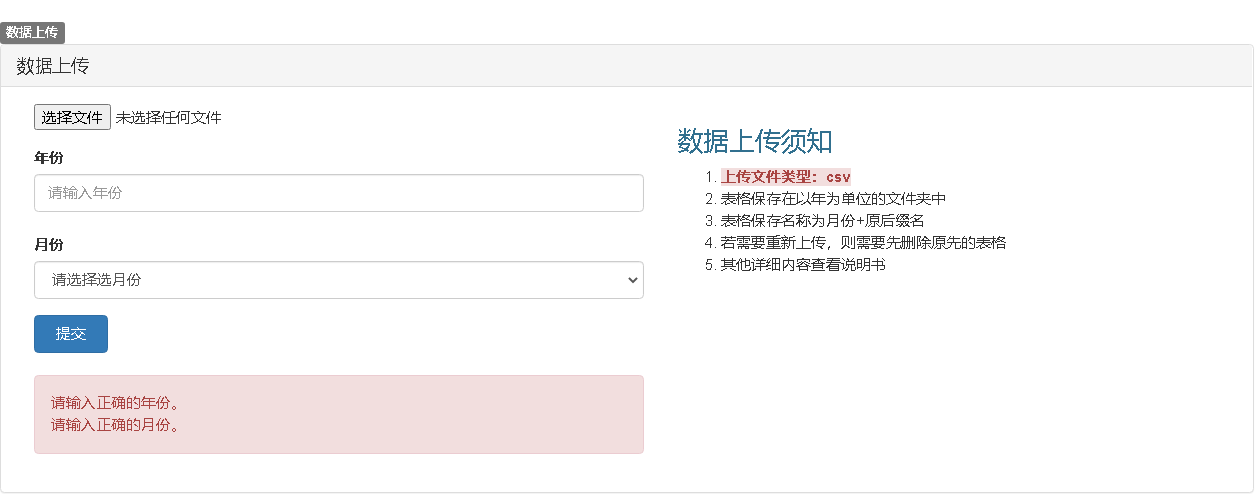
\includegraphics[width=0.7\linewidth]{pic/screenshot015}
	\caption{未选择年份或月份}
	\label{fig:screenshot015}
\end{figure}

实现方式与\ref{fileerror}类似。
\paragraph{\thesubsubsection.3 文件已存在}\ \\

若选择的年份和月份已存在数据,则警告用户文件已存在:
\begin{figure}[H]
	\centering
	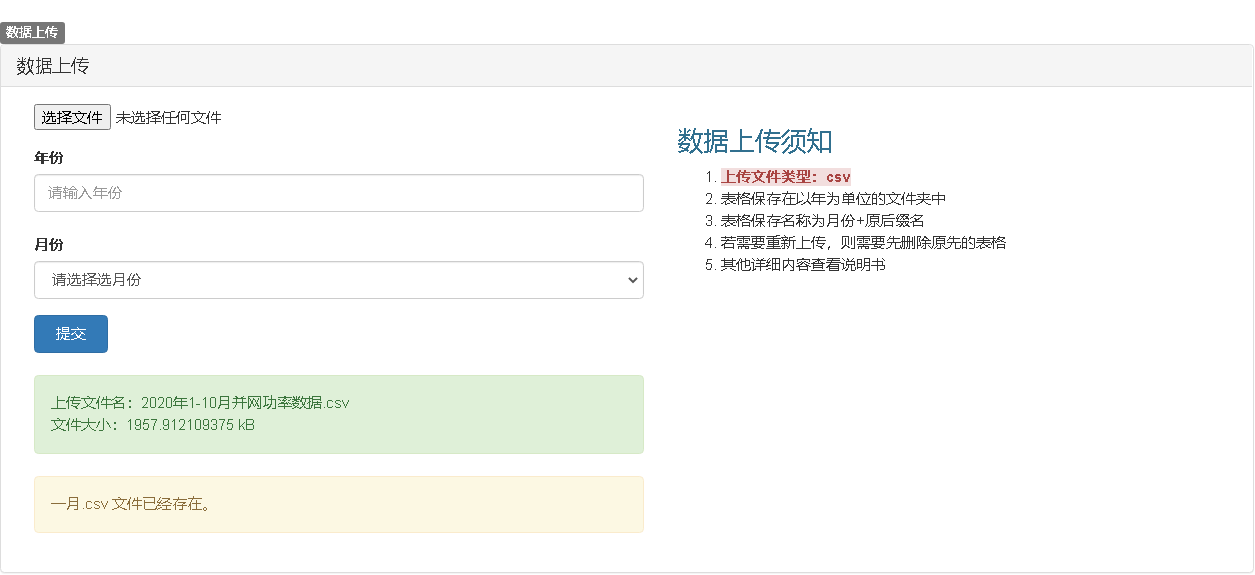
\includegraphics[width=0.7\linewidth]{pic/screenshot018}
	\caption{文件已存在}
	\label{fig:screenshot018}
\end{figure}

文件存在警告提示整体流程如图\ref{文件存在校验},其php代码如\textit{附录B-系统功能软件平台-数据层-文件已存在}所示。
\begin{figure}[H]  
	\centering
	\scriptsize  
	\begin{tikzpicture}[node distance=2cm,]
		\node (start) [startstop] {文件存在校验};
		\node (in1) [io, below of=start,] {传入文件};
		\node (pro1) [process, below of=in1, align=center] {遍历数据库查找该文件};
		\node (dec1) [decision, below of=pro1,yshift=-0.5cm, align=center] {文件已存在};
		\node (stop2) [startstop, left of=dec1,xshift=-2cm, align=center] {显示文件存在\\警告,终止上传};
		\node (stop1) [startstop, right of=dec1,xshift=2cm, align=center] {无需提示,\\文件正常上传};
		\draw [arrow](start) -- (in1);
		\draw [arrow](in1) -- (pro1);
		\draw [arrow](pro1) -- (dec1);
		\draw [arrow](dec1) -- node[anchor=south,above=1mm] {否}(stop1);
		\draw [arrow](dec1) -- node[anchor=south,above=1mm] {是}(stop2);
	\end{tikzpicture}
	\caption{文件格式校验流程图}
	\label{文件存在校验}
\end{figure} 

\subsection{数据库}
\subsubsection{月度电网数据导入}
网站需要能方便地上传月度数据,在此定义导入数据的格式和方法。

为了储存大量电厂原始数据,使用\textbf{sql}作为数据库。但对于电厂原始数据的上传,规定使用csv格式。

下面定义传入格式的表头:
\paragraph{\thesubsubsection.1 风光预测考核}\ \\
\begin{lstlisting} [language=Python]
	time_stamp,time_value,day_pred,rt_pred,real_complete
\end{lstlisting}
其中必须存在的列为:
\begin{enumerate}
	\item day\_pred,日预测数据
	\item rt\_pred,实时预测数据
	\item real\_complete,完整的实际功率数据
\end{enumerate}

其余列中,time\_stamp为Unix Timestamp,为场站人员从数据库中导出的原始数据;time\_value为Unix时间戳的转换数据,是一个我们日常使用的日期格式,如2022年3月29日 15:48:46。

\paragraph{\thesubsubsection.2 一次调频考核}\ \\
\begin{lstlisting} [language=Python]
	time,out,qe,fre
\end{lstlisting}
其中必须存在的列为:
\begin{enumerate}
	\item time,时间戳,可以为Unix Timestamp或日常使用的时间格式
	\item out,机组实际出力数据
	\item qe,机组理论出力数据
	\item fre,系统频率数据
\end{enumerate}

\subsubsection{数据储存与导出}
为了方便数据传输,网站使用json的格式进行数据传输。json是一种数据交换格式,其具有轻量化,易于人阅读、编写,易于及其解析的特定,因此方便在多个函数之间进行传输。一般来说,json对象是一个的“‘键/值’对”集合,如我们常用的数组可以看作是一种特殊的json:其“键”为从0开始递增的数列。下面例子是一个json对象:

\begin{lstlisting} [language=Python]
	{"name": "Ysx", "age": 22, "address": {"country" : "china", "code": "+86"},
		"name": "Zjj", "age": 25, "address": {"country" : "china", "code": "+86"}}
\end{lstlisting}

下面对每一板块的json格式进行规定:

\paragraph{\thesubsubsection.1 风光预测考核}\ \\
风电预测和光伏预测考核的数据比较相同,因此使用同样的模板进行储存。



\subparagraph{\thesubsubsection.1.1 月度板块}\label{momthjsonWind}\ \\
月度详情页面需要数据为:
\begin{enumerate}
	\item 绘图:
	\begin{enumerate}
		\item 日预测准确率
		\item 日预测考核时长
		\item 日预测准确率合格线
		\item 96点功率曲线
		\item 实时预测准确率
		\item 实时预测考核时长
		\item 实时预测准确率合格线
	\end{enumerate}
	\item 制表:
	\begin{enumerate}
		\item 日预测准确率
		\item 日预测考核时长
		\item 实时预测准确率
		\item 实时预测考核时长
	\end{enumerate}
\end{enumerate}

因此对传入风光预测考核的json数据进行如下格式规定(具体内容以“...”代替):
\begin{lstlisting} [language=php]
	{"文件生成时间":...,
		"考核结果计数":
		{"实时预测":{"考核合格":...,"考核不合格":...},
			"日预测":{"考核合格":...,"考核不合格":...}},
		"作图数据":
		{"日预测准确率":[...],"日预测考核时长":[...],"时间":[...],
			"Axis":{"yAxis":{"yAxis_96_min":[...],"yAxis_96_max":[...],
					"yAxis_main_min":...,"yAxis_main_max":...},
				"xAxis":{"功率曲线时间轴":[...],"xAxis_main_max":...}},
			"实时预测准确率1":[...],"实时预测准确率2":[...],"实时预测准确率3":[...],
			"实时预测准确率4":[...],"实时预测准确率5":[...],"实时预测准确率6":[...],
			"dataset_96":[{"真实96点曲线":[...],"预测96点曲线":[...]}],
			"合格线":{"日预测准确率合格线":...,"实时预测准确率合格线":...}},
		"作表数据":
		{"时间":[...],"日预测准确率":[...],"日预测考核时长":[...],
			"实时预测准确率1":[...],"实时预测考核时长1":[...],"实时预测准确率2":[...],
			"实时预测考核时长2":[...],"实时预测准确率3":[...],"实时预测考核时长3":[...],
			"实时预测准确率4":[...],"实时预测考核时长4":[...],"实时预测准确率5":[...],
			"实时预测考核时长5":[...],"实时预测准确率6":[...],"实时预测考核时长6":[...]}}
\end{lstlisting}
%	\arabic{\subparagraph}
\subparagraph{\thesubsubsection.1.2 主页面(年度板块)}\ \\
主页面需要的数据为:
\begin{enumerate}
	\item 绘图:
	\begin{enumerate}
		\item 实时预测考核时长
		\item 	日预测考核时长
		\item 	总考核时长
	\end{enumerate}
	\item 制表:
	\begin{enumerate}
		\item 日预测/实时预测合格次数
		\item 	日预测/实时预测不合格次数
		\item 	日预测/实时预测合计次数
	\end{enumerate}
\end{enumerate}

读取月度板块中储存的每个月的json数据,通过对相应的数值进行加减即可获得上述所需数据。
\paragraph{\thesubsubsection.2 一次调频积分电量考核}\label{Pjsonmonth}

\subparagraph{\thesubsubsection。2.1 月度详情页面、日板块}\ \\
一次调频积分电量考核的月度详情页面需要如下内容:
\begin{enumerate}
	\item 考核金额详细数据
	\item 考核动作详细数据
\end{enumerate}

因此对一次调频积分电量考核板块月度详情页面的json做如下格式规定(具体内容以“...”代替):

\begin{lstlisting} [language=php]
	{"文件生成时间":...,
		"考核结果计数":
		{"考核合格":...,"考核不合格":...,"无需考核":...},,
		"作图数据":
		{"dataset":[...]
			"Axis":{"yAxis":{"yAxis_out_min":[...],"yAxis_out_max":[...],"yAxis_fre_min":...,"yAxis_fre_max":...}}},
		"作表数据":
		{"时间":[...],"考核结果":[...]},
		"每分钟详细数据":[...]}
\end{lstlisting}

\subparagraph{\thesubsubsection.2.2 主页面}\ \\
一次调频积分电量考核的主页面需要如下内容:
\begin{enumerate}
	\item 考核金额数据
	\item 考核动作数据
\end{enumerate}

读取月度板块中储存的每个月的json数据,通过对相应的数值进行加减即可获得上述所需数据。

\subsubsection{数据传输}


jQuery是一个JavaScript库,其极大地简化了JavaScript的编程。在HTML中,前端和后端使用Ajax进行通讯。jQuery对Ajax进行了高级封装:需要读取json文件时,可以向服务器发送GET请求,在请求的同时指定dataType为json,便可以请求服务器返回对应路径下的json对象。将该方法封装为函数,其JavaScript代码如\textit{附录B-系统功能软件平台-数据库-数据传输}所示。函数返回结果为JavaScript Object,可以直接在绘图脚本中进行调用。

\subsection{运行环境}
\subsubsection{应用服务器部署}
系统在腾讯云服务器上进行系统部署,主要运行环境为Apache 2.4.39、MySQL 5.7.26和PHP 7.3.4nts。运行环境通过小皮面板进行部署,同时也部署了FTP服务器,方便进行系统运行维护和调试。
\begin{figure}[H]
	\centering
	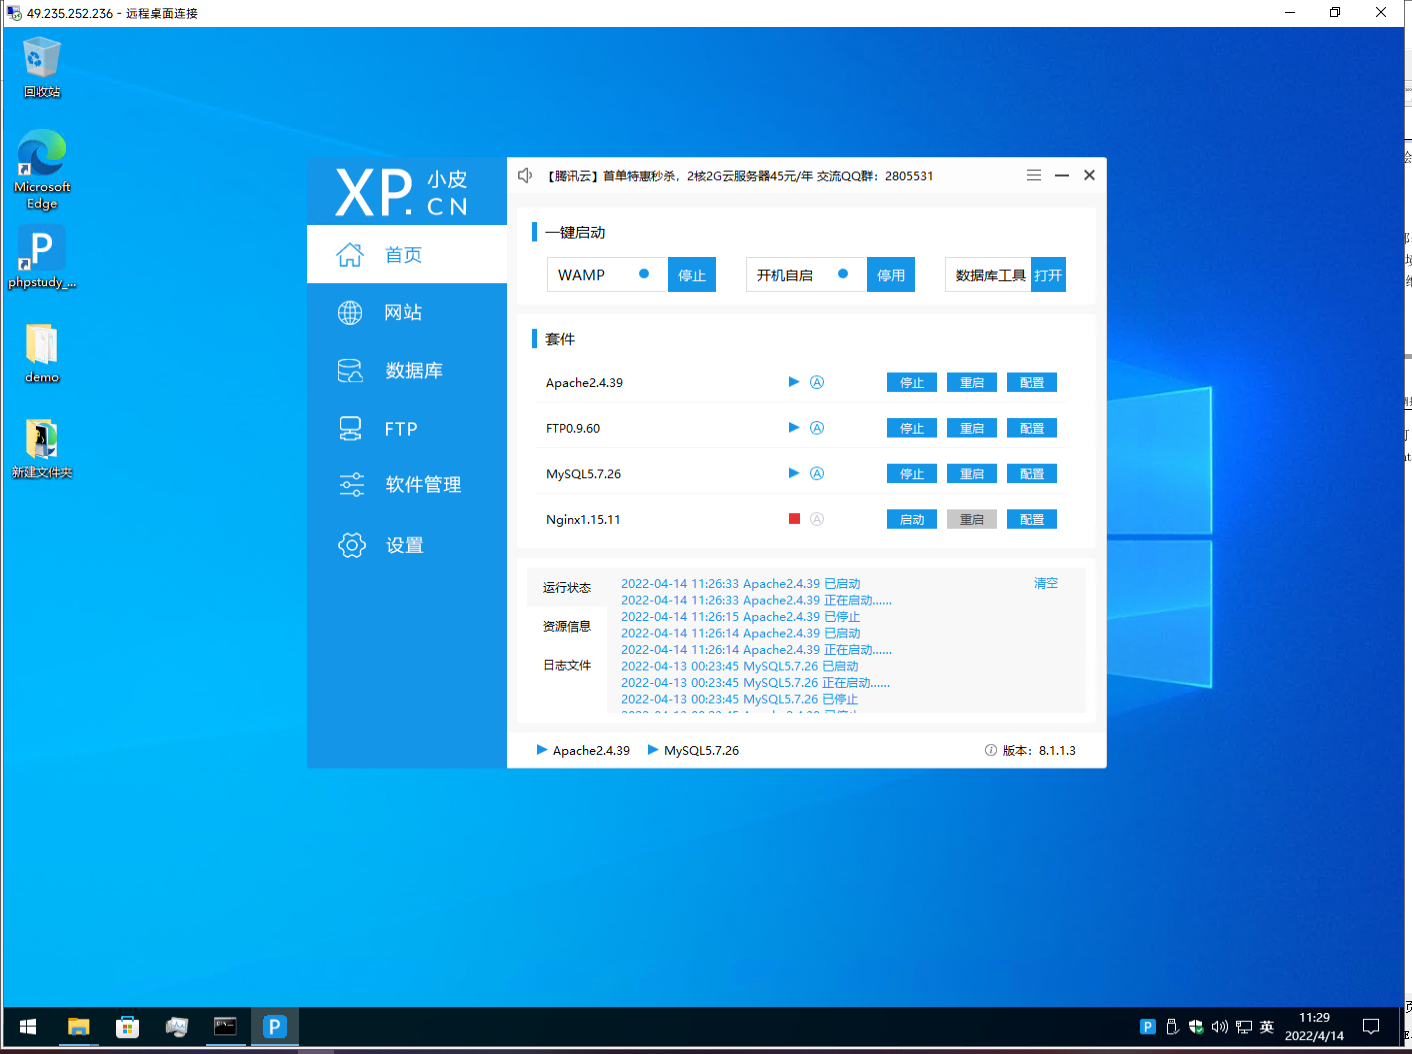
\includegraphics[width=0.7\linewidth]{pic/screenshot022}
	\caption{云服务器部署情况}
	\label{云服务器部署情况}
\end{figure}

由于所购买的云服务器具有公网IP,因此在外网中可以直接通过公网IP+端口进行访问。

\subsubsection{域名绑定}
在访问网站时,使用IP+端口进行访问往往不容易记住,因此需要进行域名绑定。

在DNS记录中,若需要将域名指向云服务器,可以使用A记录;若将域名指向另一个域名,则使用CNAME记录。此处由于是将域名指向云服务器,因此选择A记录。

\begin{figure}[H]
	\centering
	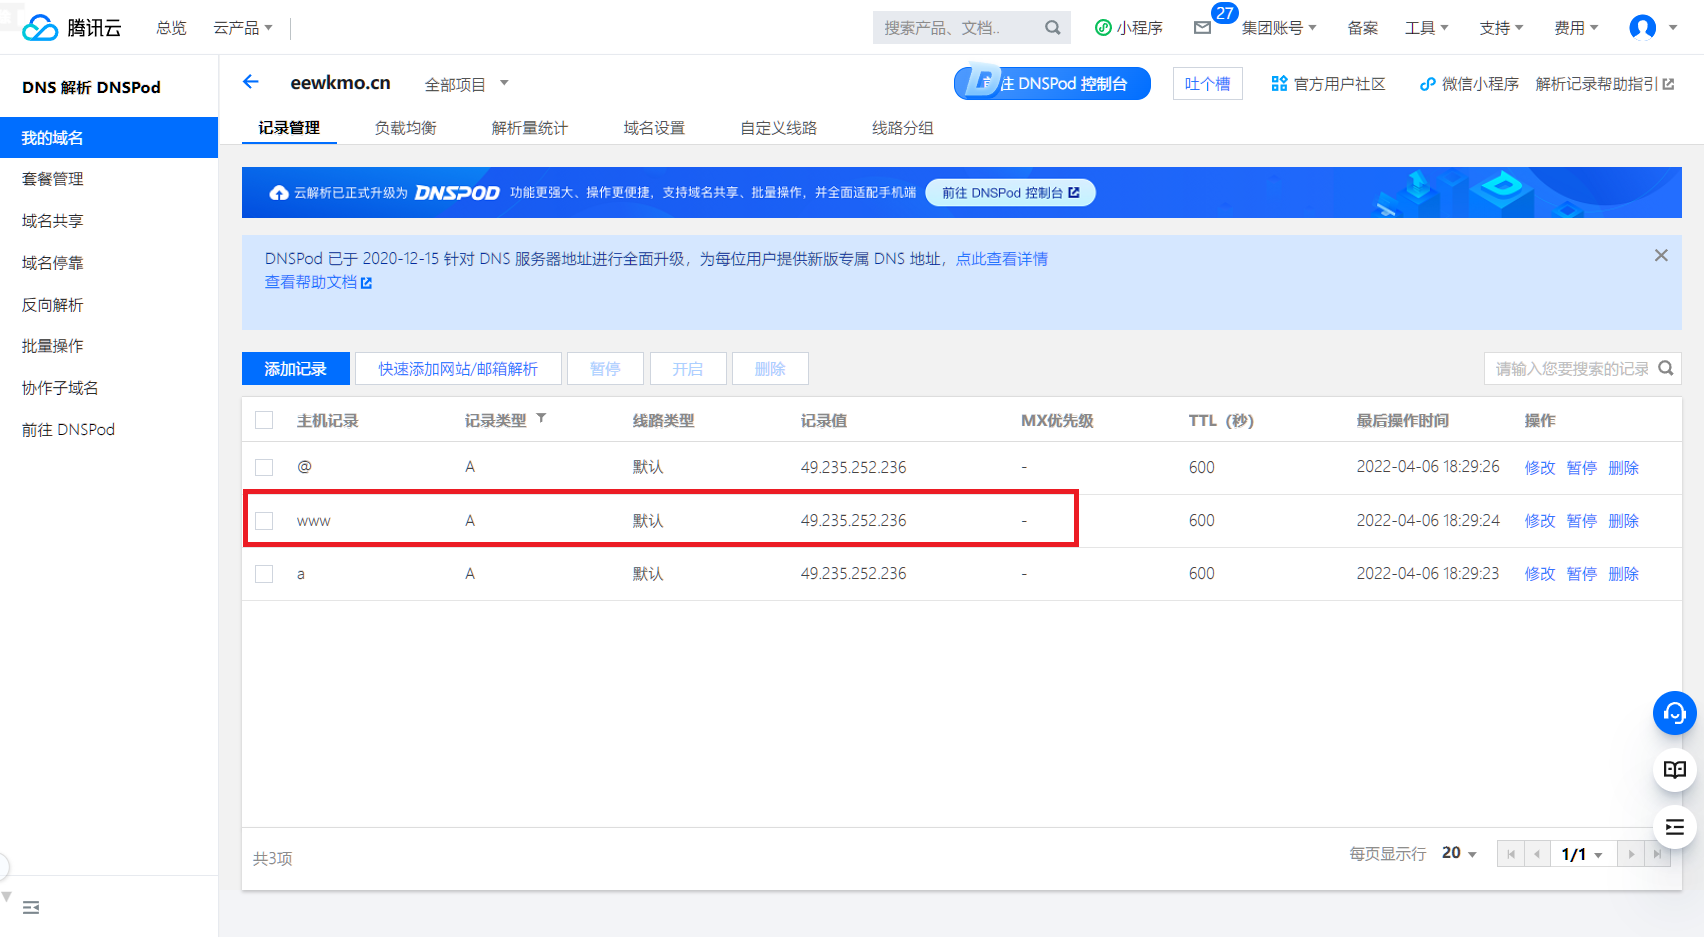
\includegraphics[width=0.7\linewidth]{pic/screenshot025}
	\caption{将域名与IP进行A记录}
	\label{fig:screenshot025}
\end{figure}

记录完成后,即可通过域名直接访问系统。

\subsection{小结}
本章的研究内容主要是平台的软件平台。系统的硬件平台分为应用服务器和数据库服务器。在硬件平台的基础上,系统的软件平台整体结构可划分为6大部分:运行环境、数据库、数据层、业务层、控制层与前端UI。

其中运行环境主要包括两台服务器,其分为应用服务器与数据库服务器。数据库使用MySQL进行数据储存,并规定了数据储存的格式。数据层提供了数据上传的接口与页面,同时也提出了三种异常处理方式。业务层主要实现考核数据计算,用户可以手动调用计算脚本进行考核数据计算,也可以将计算功能设置为系统自动任务,在设定的时间自动执行。控制层主要实现绘图和指标功能,其中,绘图功能采用echarts库进行,实现了自动缩放、重新绘制、数据切换等功能;制表使用JavaScript方法,同时对该方法进行了封装,以方便调用。前端UI主要使用html书写,使用了bootstrap库,bootstrap样式和jQuery库,实现了手风琴切换、导航栏、徽标等样式和功能。






\newpage
\section{一次调频考核}
\subsection{概述}
一次调频是指由电网负荷实时变化使得电网频率发生一定幅度的波动后,控制系统自动增减机组组发电功率,以抑制电网频率波动变化,从而达到稳定电网频率的目的\upcite{2010}。



调频是一个需要统筹调度和各个机组相互协调的问题。各级电厂在调频过程中不允许“各自为政”的情况出现。并且于经济性考虑,调频与运行费用的关系密切:调频是通过调整机组的输出功率来稳定系统频率,而机组输出功率改变,机组消耗的燃料及费用就随着改变\upcite{dlxtzdh}。

但随着电力市场改革的不断深入,厂网分开后,机组考核管理难度日益增大。而且近年来,小型发电机组的并网、新能源机组并网,这些机组都不如大型机组一样具有较强的一次调频能力\upcite{jyzzdnkzhxdccn},削弱了整个系统的一次调频性能,导致在事故恢复过程中稳态频率过低,不利于系统安全\upcite{20142jzyctp}。因此,一套准确的一次调频考核机制对系统保持良好的一次调频能力,增加电网运行质量具有重要意义。

\subsection{一次调频过程}
在电力系统中,发电机组发出的有功功率与负荷消耗的有功功率处于一个动态平衡状态\upcite{电力系统分析},即$ P_{G}-P_{D}=0 $。对发电机组而言,当发电机输出的电磁功率大于原动机输出的机械功率时,其制动力矩大于驱动力矩,此时频率下降;反之,频率上升。假设有如图\ref{发电机原动机负荷}的系统,其中原动机输出功率为恒定,当系统正常运行时,发电机功率$ P_{G} $与负荷功率$ P_{D} $相等;若在某一时刻负荷增多,则发电机功率也同时增大,但由于原动机输出功率恒定,此时制动力矩大于驱动力矩,从而导致系统频率下降。
\begin{figure}[H]
	\centering
	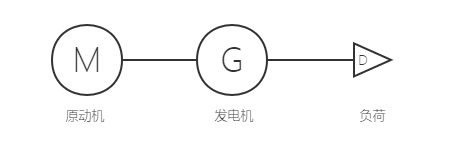
\includegraphics[width=0.7\linewidth]{pic/发电机原动机负荷}
	\caption{原动机-发电机-负荷的简单系统}
	\label{发电机原动机负荷}
\end{figure}

电网频率正常情况下仅在$ \pm 0.2\sim\pm0.5 $之间波动,若频率波动大于该值,则会造成事故。由于系统中负荷是实时变化的,因此对于发电机组而言,需要有一定的手段抑制由于负荷变化而导致的频率变化,一次调频就是其中一种较为方便有效方法。

一次调频过程如图\ref{一次调频过程}所示:
\begin{figure}[H]  
	\centering
	\scriptsize  
	\begin{tikzpicture}[node distance=2cm,]
		\node (start) [startstop] {电力系统};
		\node (in1) [io, below of=start,] {系统频率变化$ \Delta f $};
		\node (pro1) [process, below of=in1, ] {计算期望发电量$ P $};
		\node (pro2) [process, below of=pro1, ] {调速器动作};
		\node (pro3) [process, below of=pro2, ] {机组根据调速器动作发出功率};
		\draw [arrow](start) -- (in1);
		\draw [arrow](in1) -- (pro1);
		\draw [arrow](pro1) -- (pro2);
		\draw [arrow](pro2) -- (pro3);
		\draw [arrow](pro3.east) -- node[]{}($(pro3.east) + (1.05,0)$) |- ($(pro1.east)+(1.6,0)$) |- ($(pro1.east)+(0,0)$);
		\draw [arrow](pro2.west) -- node[]{}($(pro2.west) - (1.5,0)$) |- ($(start.west)-(1.6,0)$) |- ($(start.west)+(0,0)$);
	\end{tikzpicture}
	\caption{一次调频过程}
	\label{一次调频过程}
\end{figure} 

当系统中用户负荷增加时,原动机提供的驱动力矩小于负荷带来的制动力矩,导致系统频率下降;此时调速器动作,增大原动机气门开度,使得原动机转速上升,从而提高了原动机的机械功率;原动机机械功率上升,使得发电机电磁功率上升,驱动力矩与制动力矩趋于平衡,使系统频率稳定在一个与正常运行频率偏差较小的值上\upcite{电力系统自动化}。
%	
%	现今机组一般使用自动发电控制系统(AGC)进行一次调频控制。在区域电网联合成的大电网中常用的控制方法为分区调频法,其调频方程为:
%	\begin{equation}\label{key}
%		ACE=K\Delta f+\Delta P_{tie}
%	\end{equation}
%	
%	式中,$ \Delta P_{tie} $为分区联络线上的功率变化。
%	
\subsection{评判指标}
“两个细则”中提出了2个考核指标:合格率和投入率\upcite{南方区域发电厂并网运行管理实施细则(2020年版)}。

\subsubsection{一次调频合格评判指标}	
考核分为两步:1、当系统频率超过死区时,机组出力应与频率偏差方向相反,记为合格。2、实际动作积分电量与理论动作积分电量的比值小于规定值,记为合格。若二者均合格则该时段内的动作合格,反之记为不合格。考核时间分辨率为1分钟,实际动作积分电量与理论动作积分电量的比值规定值为0.35。

根据《水轮机调节系统并网运行技术导则》\upcite{20132013水轮机调节系统并网运行技术导则},一次调频理论动作积分电量$ Q_{e} $可通过下列公式计算\upcite{水电机组一次调频理论积分电量计算方法}:
\begin{equation}\label{yctp1}
	Q_{e}=\int_{t_{0}}^{t_{1}} \Delta P(\Delta f,t)\mathrm{d}t
\end{equation}

\begin{equation}\label{yctp2}
	\Delta P(\Delta f,t)=P_{n}\dfrac{\Delta f(t)}{f_{n}}\dfrac{1}{e_{p}}
\end{equation}

\begin{equation}\label{yctp3}
	\Delta f(t)=|f_{t}-f_{n}|-f_{\texttt{人工死区}}
\end{equation}

式中,$ \Delta P $为实际功率变化量;$ \Delta f $为电网频率变化超过人工死区的频率差,该死区在汽轮机机组中为0.03Hz,水轮机为0.05Hz;$ P_n $为额定有功出力;$ f_n $为额定频率,50Hz;$ e_{p} $为机组永态转差系数,在后续计算取$ e_{p}=0.04 $;$ t_0 $,$ t_1 $分别为一次调频起始和结束时刻。

一次调频实际动作积分电量$ Q_{a} $可通过如下公式计算\upcite{李玺2018水电机组一次调频理论动作积分电量优化算法}:
\begin{equation}\label{yctp4}
	Q_{a}=\int_{t_{0}}^{t_{1}}\Delta P(t) \mathrm{d}t
\end{equation}

\begin{equation}\label{yctp5}
	\Delta P(t)=P_{a}-P_{0}
\end{equation}

式中,$ P_{a} $为机组实际出力,$P_{0}  $为积分起始时刻对应的机组实际出力。
\subsubsection{一次调频合格率}
不合格率指一定时段内的动作不合格次数与应动作总次数的百分比。相对应的,一次调频合格率=1-一次调频不合格率。可以写成如下公式:
\begin{equation}\label{yctphgl}
	R_{qualifide}=\frac{T_{up\ to\ standard}}{T_{total}}\times 100\%
\end{equation}

\subsubsection{一次调频投入率}
一次调频功能投入时间与并网运行时间的百分比为投入率,可以写成如下公式:
\begin{equation}\label{yctptrl}
	R_{in\  server}=\frac{T_{in\  server}}{T_{on\  grid}}\times 100\%
\end{equation}

\subsection{评价指标算法}
\subsubsection{一次调频合格率}
\paragraph{\thesubsubsection.1 第一步}\ \\

第一步需要判断一次调频是否动作。若动作,则计算频率差和功率差,并判断是否合格;反之则记为无需考核。其流程如图\ref{yiciliucheng1}所示:

\begin{figure}[H]  
	\centering
	\scriptsize  
	\begin{tikzpicture}[node distance=2cm,]
		\node (start) [startstop] {一次调频考核};
		\node (in1) [io, below of=start] {系统频率数据};
		\node (in2) [io, right of=in1, xshift=4cm] {机组实际出力数据};
		\node (pro1) [process, below of=in1] {系统频率变化量};
		\node (pro2) [process, below of=in2] {机组实际出力变化量};
		
		\node (dec1) [decision, below of=pro1, yshift=-2cm, align=center] {系统频率是否\\在死区内};
		\node (dec2) [decision, below of=pro2, yshift=-2cm, align=center] {两变化量符号\\ 是否相同};
		
		\node (stop1) [startstop, below of=dec1,,yshift=-1cm] {无需考核};
		\node (stop2) [startstop, below of=dec2,,yshift=-1cm] {考核不合格};
		\node (stop3) [startstop, right of=dec2,,xshift=1.5cm] {考核合格};
		%连接具体形状
		\draw [arrow](start) -- (in1);
		\draw[arrow] (
		in1.west)-- node[] {} ($(in1.west) - (1.05,0)$) |- ($(dec1.west)-(0.8,0)$) -- (dec1.west);
		\draw [arrow](in1) -- (pro1);
		\draw [arrow](in2) -- (pro2);
		\draw [arrow](pro1.south) -- (dec2.west);
		\draw [arrow](pro2) -- (dec2);
		\draw [arrow](dec2) -- node[anchor=east,above=0.5mm] {否} (stop3);
		\draw [arrow](dec2) -- node[anchor=south,above=-1mm,left=0.5mm] {是} (stop2);
		\draw [arrow](dec1) -- node[anchor=east] {是} (stop1);
		\draw [arrow](dec1) -- node[anchor=south,above=-1mm] {否} (dec2);
		
		
	\end{tikzpicture}
	\caption{第一步计算流程图}
	\label{yiciliucheng1}
\end{figure}  




\paragraph{\thesubsubsection.2 第二步}\ \\

第二部在第一步的基础上,计算实际出力积分电量和理论出力积分电量,并判断二者之比是否在规定值以内。其流程如图\ref{yiciliucheng2}所示:
\begin{figure}[H]  
	\centering
	
	\scriptsize  
	
	%像素点,用于连接转移线
	\begin{tikzpicture}[node distance=2cm]
		%定义流程图具体形状
		\node (start) [startstop] {一次调频考核};
		\node (in1) [io, below of=start] {系统频率数据};
		\node (in2) [io, right of=in1, xshift=3cm] {机组实际出力数据};
		\node (in3) [io, right of=in2, xshift=3cm] {机组理论出力数据};
		\node (pro2) [process, below of=in2] {机组实际积分电量};
		\node (pro3) [process, below of=in3] {机组理论积分电量};
		
		\node (dec1) [decision, below of=pro1, yshift=-2.5cm, align=center] {系统频率是否\\在死区内};
		\node (dec2) [decision, below of=pro2, xshift=2.5cm,yshift=-2.5cm, align=center] {二者比值是否\\小于规定值};
		
		\node (stop1) [startstop, below of=dec1,,yshift=-1cm] {无需考核};
		\node (stop2) [startstop, below of=dec2,,yshift=-1cm] {考核不合格};
		\node (stop3) [startstop, right of=dec2,,xshift=1.5cm] {考核合格};
		%连接具体形状
		\draw [arrow](start) -- (in1);
		\draw [arrow](in2) -- (pro2);
		\draw [arrow](in3) -- (pro3);
		\draw [arrow](in1) -- (dec1);
		\draw [arrow](pro2.south) -- (dec2.north);
		\draw [arrow](pro3.south) -- (dec2.north);
		\draw [arrow](dec2) -- node[anchor=east,above=0.5mm] {否} (stop3);
		\draw [arrow](dec2) -- node[anchor=south,above=-1mm,left=0.5mm] {是} (stop2);
		\draw [arrow](dec1) -- node[anchor=east] {是} (stop1);
		\draw [arrow](dec1) -- node[anchor=south] {否} (dec2);
	\end{tikzpicture}
	\caption{第二步计算流程图}
	\label{yiciliucheng2}
\end{figure}  
\paragraph{\thesubsubsection.3 第三步}\ \\

最后综合上述两步,若一二步中有一步或以上不合格,则记为不合格,反之该次一次调频考核记为合格。
\paragraph{\thesubsubsection.4 计算时间段内的合格率}\ \\
一次调频合格率考核时间间隔为一分钟一次。若取时间段为一日,由\ref{yctphgl}可得:
\begin{equation}\label{key}
	R_{qualifide}=\frac{T_{up\ to\ standard}}{1440}\times 100\%
\end{equation}

其中$ T_{up\ to\ standard} $为本日内正确动作的次数。由此可计算出本日内一次调频考核合格率。


\subsubsection{一次调频投入率}
一次调频投入率考核考核为一个月一次,根据\ref{yctptrl}即可计算出一次调频投入率。

\subsection{算法的PHP实现}
\subsubsection{第一步}
根据图\ref{yiciliucheng1},第一步需要判断频率是否在死区内,以及频率变化量与出力变化量的符号是否相同。据此可以分别将两部分封装成函数:

\begin{enumerate}
	\item 判断频率是否在死区:将该步骤封装为如\textit{附录B-一次调频算法-第一步-频率死区}中的函数,以方便调用。
	
	\item 频率变化量与出力变化量的符号是否相同:该步骤封装为如\textit{附录B-一次调频算法-第一步-符号判断}中的函数。
\end{enumerate}

\subsubsection{第二步}

根据图\ref{yiciliucheng2},第二步为计算机组实际积分电量与理论积分电量,并判断其比值是否在规定范围内。第二步可以封装为如\textit{附录B-一次调频算法-第二步-主程序}中的函数。其中,一次调频理论积分电量可以由\textit{附录B-一次调频算法-第二步-理论积分电量}的代码计算,一次调频实际积分电量可以由\textit{附录B-一次调频算法-第二步-实际积分电量}的代码计算,也可以直接传入计算得出的理论功率,再使用主程序中的代码计算。

\subsubsection{第三步}
第三步获取上述两步结果,若二者均为合格即记本次一次调频考核合格,反之记为不合格。将该方法封装后如\textit{附录B-一次调频算法-第三步}的代码所示。封装函数传入的参数中,qualified1为第一步结果,qualified2为第二步结果。

\subsection{算例演示}
本节使用2017年4月7日16时小湾电厂\#4F号机组的有功功率数据和云南异步联网虚拟厂站云南电网GPS频率数据进行算例演示。数据共计3600行,分为四列,时间、实际功率、理论功率,系统频率,储存在“一次调频算例.csv”中。

将数据放入计算公式:
\begin{lstlisting} [language=php]
	require_once 'algorithm.php';
	
	$csv_1_path = './一次调频算例.csv';
	$array=csv_read_and_encode($csv_1_path);
	
	$fre_array = $array['fre'];
	$xiaowan_array = $array['xiaowan'];
	$pred_array = $array['qe'];
	$time=$array['time'];
	
	$res=PFM_main($fre_array,$xiaowan_array,$pred_array,$time,0.03);
	
\end{lstlisting}

可以得到如下结果:
\begin{figure}[H]
	\centering
	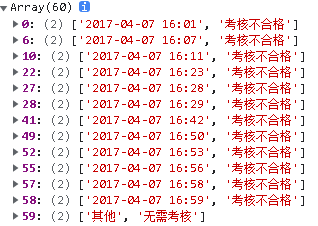
\includegraphics[width=0.5\linewidth]{pic/screenshot024}
	\caption{一次调频算例结果}
	\label{fig:screenshot024}
\end{figure}

\subsection{小结}
本章的研究内容主要是通过分析系统频率数据、机组功率实际数据对机组一次调频性能进行考核。

根据“两个细则”,本章提出了2个考核指标,分别为:合格率、投入率,其中功率预测又分为合格率和考核时长两部分。并对2个指标设计了相应的算法。

本章通过使用2017年4月7日16时小湾电厂\#4F号机组的有功功率数据和云南异步联网虚拟厂站云南电网GPS频率数据验证了算法的准确性和可行性,但同时也发现,当电网受到扰动时,算例中机组并不能很好地按照规定完成一次调频动作,需加强机组对一次调频能力的考核和检测。


\section{风光预测考核}

\subsection{概述}
风、光具有不确定性、高间歇性和不可调度性\upcite{刘云2019基于双参数最小二乘支持向量机}。如今,大量新能源场站逐渐进入从独立发电转入到并网发电的过程中,这些新能源并网机组对电力系统的稳定运行提出了新的要求。为了降低风光发电并网对电力系统的冲击、提高风功率与光伏利用率,就需要对新能源机组和电网做出合理的统筹调度\upcite{孙成胜2020一种改进的灰色}。短期功率预测这一概念能有效降低新能源并网对电网的不理影响\upcite{kumpf2017visualizing,王昕2016基于},并且可以作为电网调度和电站维护的参考\upcite{黎静华2017基于,王要强2016光伏发电系统输出功率特性分析及其平滑控制研究,王守相2012基于灰色神经网络组合模型的光伏短期出力预测,毕锐2016基于模糊}。

预测模型一般分为物理模型\upcite{warrington2017low},统计模型\upcite{yan2017forecasting}和混合模型\upcite{yan2016novel}。其中物理模型基于天气预报、风电场地形等参数的详细物理建模来实现预测;统计模型则基于历史数据时间序列实现。场站侧常采用统计模型进行预测。

南方电网为保障南方区域电力系统的安全、优质、经济运行,对风电站和光伏电站进行并网调度规范管理,同时针对风光发电的特点对二者的调度运行管理提出一系列考核方法。

\subsection{评判指标}
在南方电网“两个细则”中,虽然风电预测和光伏预测是分开讨论,但其核心算法相同,因此本章将二者合并。

风光预测评判指标共有3大类\upcite{南方区域光伏电站并网运行及辅助服务管理实施细则(2020年版),南方区域风力发电场并网运行及辅助服务管理实施细则(2020年版)}:
\subsubsection{上报情况}
\begin{enumerate}
	\item 风电站与光伏电站需按要求完成数据报送和上传历史数据。未达要求则即为不合格。
	\item  风电站与光伏电站需及时按要求上报装机容量、可用容量或调度系统要求的其他信息,漏报或迟报则按不合格处理。
\end{enumerate}

\subsubsection{日预测}
日前预测是指场站对未来24小时,即下一日0:00至23:45的新能源功率进行预测。其时间分辨率为15分钟,即使用96点功率曲线进行计算。对于光伏电站,考核合格线为85\%;对于风电站,考核合格线为80\%。日预测考核计算公式如下:
%	
%	
%	(1)日预报上报率应达到100\%
%	
%	(2)日预报准确率低于合格基准线的,按以下公式考核日预报准确率按日进行统计、考核。

\begin{equation}\label{pre_wind_day}
	\texttt{日准确率}=(1-\dfrac{\sqrt{\sum\limits_{i=1}^{n}(P_{Mi}-P_{Pi})^2}}{Cap\sqrt{n}})
\end{equation}

其中:$ P_{Mi} $为i时刻的实际功率,$ P_{Pi} $为i时刻的日预报值,Cap为总装机容量,n=96为样本个数。

若考核不合格,则日准确率考核电量=(合格基准线-日准确率)$ \times \texttt{Cap}\times 1 $(小时)

\subsubsection{实时预测}
实时预测是指自上报时刻起未来4小时的预测预报,其时间分辨率为15分钟,即使用16点功率曲线进行计算。对于光伏电站,考核合格线为90\%;对于风电站,考核合格线为85\%。实时预测考核计算公式如下:

%	(1)实时预报上报率应达到100\%
%	
%	(2)实时预报准确率低于合格基准线的,按以下公式考核实时预报准确率按日进行统计、考核。
\begin{equation}\label{pre_wind_rt}
	\texttt{实时准确率}=(1-\dfrac{\sqrt{\sum\limits_{i=1}^{n}(P_{Mi}-P_{Pi,t})^2}}{Cap\sqrt{n}})
\end{equation}

其中:$ P_{Mi} $为i时刻的实际功率,$ P_{Pi,t} $为i时刻的实时预报值,Cap为总装机容量,n=16为样本个数。

若考核不合格,则实时准确率考核电量=(合格基准线-实时准确率)$ \times \texttt{Cap}\times 1 $(小时)



\subsection{评价指标算法}
\begin{enumerate}
	\item	日预报
	
	计算上报率$ \rightarrow $计算日准确率$ \rightarrow $计算日准确率考核电量
	
	\item 实时预报
	
	计算上报率$ \rightarrow $计算实时准确率$ \rightarrow $计算实时准确率考核电量
	
\end{enumerate}
\begin{figure}[H]  
	\centering
	
	\scriptsize  
	
	%像素点,用于连接转移线
	\begin{tikzpicture}[node distance=2cm]
		%定义流程图具体形状
		\node (start1) [startstop] {日预报};
		\node (in1) [io, below of=start1] {实际功率};
		\node (in2) [io, below of=in1] {预报功率};
		\node (pro1) [process, below of=in2,] {计算上报率};
		\node (pro2) [process, below of=pro1] {计算日准确率};
		\node (pro3) [process, below of=pro2] {计算日准确率考核电量};
		\node (stop1) [startstop, below of=pro3]{日预报考核结束};
		
		\node (start2) [startstop, right of=start1, xshift=4cm] {实时预报};
		\node (in3) [io, below of=start2] {实际功率};
		\node (in4) [io, below of=in3] {预报功率};
		\node (pro4) [process, below of=in4,] {计算上报率};
		\node (pro5) [process, below of=pro4] {计算实时准确率};
		\node (pro6) [process, below of=pro5] {计算实时准确率考核电量};
		\node (stop2) [startstop, below of=pro6]{实时预报考核结束};
		
		
		%连接具体形状
		\draw [arrow](start1) -- (in1);
		\draw [arrow](in1) -- (in2);
		\draw [arrow](in2) -- (pro1);
		\draw [arrow](pro1) -- (pro2);
		\draw [arrow](pro2) -- (pro3);
		\draw [arrow](pro3) -- (stop1);
		\draw [arrow](start2) -- (in3);
		\draw [arrow](in3) -- (in4);
		\draw [arrow](in4) -- (pro4);
		\draw [arrow](pro4) -- (pro5);
		\draw [arrow](pro5) -- (pro6);
		\draw [arrow](pro6) -- (stop2);
		
	\end{tikzpicture}
	\caption{计算流程图}
	\label{fengdianyuceliucheng}
\end{figure} 

\subsection{算法的PHP实现}

风光预测二者的算法差别仅在合格基准线,因此将二者放在同一模块中进行计算,仅需传入不同的参数即可。根据\ref{pre_wind_day}和\ref{pre_wind_rt},风光预测的核心计算公式封装代码见\textit{附录B-风光预测考核-预测考核公式}。

函数传入参数中,real为实际功率数据,pred为预测功率数据,base为考核准确率合格线,cap为机组装机容量,mode为模式选择,分为日考核(day)和实施考核(rt)。返回值中,预测准确率和考核时长均保留4位小数。

在上述封装的函数中,若考核合格,则会返回一个负的考核时长,在做图做表的时候需要将其替换为“-”,使用\textit{附录B-风光预测考核-考核时长格式化}中的代码实现该功能。其中,传入参数qualified为考核结果数据。


\subsection{算例演示}
本节使用风电预测进行算例演示。由于上报情况需要场站数据支持,本算例中仅演示功率预测部分。

本节使用三月山风电场2020年9月6日0:00至23:45共计24小时的并网功率、短期预测功率、超短期预测功率计算。此组数据储存在风光预测算例.php中。

\subsubsection{日预测}

\begin{lstlisting} [language=php]
	require_once 'algorithm.php';
	var_dump(power_forecast_algorithm($real, $pred, 80, 1));
\end{lstlisting}

其结果为:
\begin{figure}[H]
	\centering
	
\includegraphics[width=0.7\linewidth]{pic/screenshot008}
	\caption{日预测考核结果}
	\label{fig:screenshot008}
\end{figure}



\subsubsection{实时预测}

\begin{lstlisting} [language=php]
	require_once 'algorithm.php';
	$rt_real = spilt_array($real, 16);
	$rt_pred = spilt_array($pred, 16);
	
	$search_key = array_keys($rt_real);
	foreach ($search_key as $key) {
		var_dump(power_forecast_algorithm($rt_real[$key], $rt_pred[$key], 85, 1, 'rt'));
		echo '<br>';
	}
\end{lstlisting}
\begin{figure}[H]
	\centering
	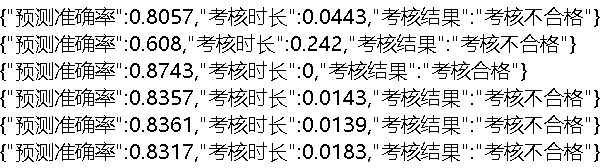
\includegraphics[width=0.7\linewidth]{pic/screenshot007}
	\caption{实时预测考核结果}
	\label{fig:screenshot007}
\end{figure}

\subsection{小结}
本章的研究内容主要是通过分析风光功率实际数据与预测数据的关系,对风光预测的准确度进行考核评估。目的是提高短期功率预测的准确度,降低新能源并网对电网的影响。

根据“两个细则”,本章提出了3个考核指标,分别为:上报情况、日功率预测、实时功率预测,其中功率预测又分为合格率和考核时长两部分。并对3个指标设计了相应的算法。

最后,本章通过三月山风电场2020年9月6日实际上报的风电功率数据验证了算法的准确性和可行性,为电网调度和电站维护提供参考数据。但从考核算例的结果中不难发现,现今场站对预测数据重视程度不足,其上传的预测数据为一条直线,并不能很好的对一天的风功率进行拟合,从而导致如算例中日预测不合格,六次实时预测也仅有一次合格。针对这一现象,电力系统需要对新能源场站加大新能源功率预测考核力度,提高场站对功率预测的重视程度,并通过一定的措施激励场站探索和使用更先进的功率预测模型。

\newpage
\section{总结与展望}

本平台在南方电网“两个细则”的基础上,提出了一次调频考核和风光预测考核的算法,并编程实现了相应的算法。在系统运行效果中可以看到,本平台可以实现单站考核数据的可视化,为场站提供了实际运行过程中的优化策略。

本平台针对分布式小容量并网机组,建立了网源分析与控制平台的通用框架结构,并对其提出了一次调频和新能源功率预测的考核算法。基于不同的应用场景,平台可较为方便地根据场站实际需求来改变业务算法,实现不同场站的需求,对场站能力进行全方面的评估。

目前,本平台最大的不足是缺乏实际数据的验证。对于风光预测考核而言,虽然现今传入的数据已达约27000行,在计算过程中也未出现错误,但可能还需要更多的数据进行测试。在一次调频考核中,实际数据仅有7200行,即2个小时的数据量,原本按照设想,我需要一个月的数据来进行一次调频考核的实际数据验证,2个小时的计算量过小,无法让系统在高压力下运行而显露出一些问题。


在未来的开发中,平台还将建立机组参数和涉网模型,形成完整的网源参数综合评估数据库;加入AGC、AVC等评估考核模型,对机组励磁、调速、一次调频等特性进行评估;加入网损优化模型,以降低网损,提高电力系统运行质量等。以上特性将成为电力系统网源协调控制系统的主要功能,为分布式小容量机组的并网提供参考和控制所需的数据基础。

%%----------------- 附录 ----------------- %%
\appendix
%	
\newpage
\section*{致谢}\addcontentsline{toc}{section}{\hspace{-1em}致谢}
本系统是去年十月的时候,莫维科老师找到我,问我是否有兴趣做一个网源协调的编程项目。虽然我家有部署一个小型服务器,在上面有许多我常用的小程序接口,但是这个项目是我第一次做综合性的大型编程项目。

其实一开始,我并不准备使用PHP编写这个平台。对我来说,PHP是一门新语言。我最常用的语言是Python,虽然不敢说精通,但是一些基本的知识还是熟练掌握的。在web框架上,Python有flask框架可以使用,我家的小型服务器上的各种接口便是基于flask编写。Python的好处在于:有许多开源的库可以选用。我常跟我带的几个师弟说:“我们编程就是复制粘贴,能不造轮子我们就不造轮子,站在巨人的肩膀上,我们才能做得更快更好。”开源库带来的好处是我不需要花时间在一些可以直接复制粘贴的地方,用计算举例:Python中有著名的numpy库,其中一个特性“广播(Broadcast)”在数组计算中是十分实用的,但在PHP中,我不得不重新将Broadcast特性人工赋予PHP的数组,使得PHP的数组可以直接相加减。这就是PHP的劣势所在。

但相对于Python而言,PHP对服务器的压力较小。老师的云服务器是1C2G,在我这种用惯了高配机子的人手中真的是束手束脚(我一直都强调,最好的优化就是换更高配的机子)。PHP很好的解决了这个问题——他足够轻量化。而且他可以和HTML、JavaScript混写,Python难以媲美的特性——在Python中若HTML需要与后端通讯,唯一的办法是选择Ajax。

在老师的帮助下,我开始了系统的编程。去年由于各方面的工作,进度较为缓慢。直到12月,我才为系统搭建了基本的框架。在1月的时候,我开始进行算法的设计。先是风光预测,然后是一次调频。其实原本还有4个项目,分别是AGC管理考核、AVC管理考核、调峰考核、电压曲线合格率考核。他们的算法都已经设计完成,但由于时间关系,系统的DEMO只选用了最具有代表性的一次调频和风光预测,其他四项将交给大一的三个学弟在大创中继续编写。

制作系统最大的困难并不是编程,而是缺少实际数据用于验证。风光预测有10个月的数据,虽然数据有缺漏,但是我还是使用深度学习对其进行了补全。但是一次调频的数据缺乏严重:仅有2个小时的数据。因此我只好使用fakedata来进行测试,这一点上是本系统目前最大的不足之处。

在长达半年的毕业设计过程中,有许多人给予了我帮助和支持。在此我首先感谢莫维科老师。从系统设计,到算法实现再到平台部署,莫老师都给予了我很多帮组。他曾经也做过类似的设计,告诉了我许多过来人才知道的坑点,让我少走了很多弯路。其次感谢我的电脑。今年这台机子在半年内只蓝屏了13次,是我玩机以来蓝屏最少的一台机子,让我少死了很多脑细胞。再者,感谢大一的两位学弟,我其实是个懒人,如果不是要带你们,我也不会去深入学习PHP,而是学到能做完这个系统的水平就了事,或者最大的可能是说服老师改用Python
。最后,感谢韦景议,每次做到不想做的时候能与你吹吹水,放松放松,玩玩游戏,都对我的心情有很好的调节作用。

毕设到这里就结束了,但是这个项目并没有结束,他还会出现在今年的大创,也希望在不久的将来能在一些分布式新能源场站中看到这个系统的身影。
\newpage
\section*{附录A}\addcontentsline{toc}{section}{\hspace{-1em}附录A}
\subsection*{全部代码}

\subsubsection*{Onedrive共享链接}

https://yuuverne-my.sharepoint.com/:f:/g/personal/yuuverne\_yuuver

ne\_onmicrosoft\_com/EvG-0BeRHChAr6hjjwobb6UB9bAsaoiWWh5

E3rBmSNIFsg?e=FYyodM

\subsection*{平台访问地址}

\subsubsection*{风光预测}
http://49.235.252.236:5000/content/Wind\&LightPowerForecast/year

.php

\subsubsection*{一次调频}

http://49.235.252.236:5000/content/PrimaryFrequencyModulation/y

ear.php

\subsubsection*{文件上传}

http://49.235.252.236:5000/content/Support/upload\_file.php

\newpage
\section*{附录B}\addcontentsline{toc}{section}{\hspace{-1em}附录B}
\subsection*{系统功能软件平台}
\subsubsection*{前端UI}
\paragraph*{导航栏}\ \\
\begin{lstlisting} [language=php]
	<nav class="navbar navbar-default" role="navigation">
	<div class="container-fluid">
	<div class="navbar-header">
	...
	</div>
	</div>
	</nav>
\end{lstlisting}
\paragraph*{面包屑导航}\ \\
\begin{lstlisting} [language=php]
	<div class="col-md-12 column">
	<ul class="breadcrumb"> 
	<li class="active"><a href="year.php">年度总览</a></li>
	<li><a href="month.php">月度详情</a></li>
	</ul>
	</div>
\end{lstlisting}
\paragraph*{手风琴切换}\ \\
\begin{lstlisting} [language=php]
	<div class="panel-group" id="accordion_1">
	<div class="panel panel-default">
	<div class="panel-heading">
	<h4 class="panel-title">
	<a data-toggle="collapse" data-parent="#accordion_1" href="#collapseOne_1">
	风光考核 考核次数
	</a>
	</h4>
	</div>
	
	<div id="collapseOne_1" class="panel-collapse collapse in">
	<div class="panel-body">
	...
	</div>
	</div>
	</div>
	</div>
\end{lstlisting}
\paragraph*{数据切换}\ \\
\begin{lstlisting} [language=php]
	<form action="./month.php" role="form" method="get" class="form-inline">
	<div class="form-group">
	<label for="name">月度数据切换</label>
	<select class="form-control" name="file_list[]" id="month">
	<option value="none" selected disabled hidden>请选择选月份</option>
	</select>
	<input type="submit" value="切换" class="btn btn-default">
	</div>
	</form>
\end{lstlisting}
\subsubsection*{控制层}
\paragraph*{dataset数据初始化}\ \\
\begin{lstlisting}[language=php]
	dataset: {
		dimensions: ['时间', '日预测准确率', '日预测考核时长', '96点曲线', '96点曲线y轴最小值', '96点曲线y轴最大值', ' 实时考核准确率'],
		source: dataset_main,
	}
\end{lstlisting}
\paragraph*{使用encode选择数据}\ \\
\begin{lstlisting}[language=php]
	encode: {
		x: '时间',
		y: '日预测准确率'
	}
\end{lstlisting}
\paragraph*{对visualmap进行配置}\label{对visualmap进行配置}\ \\
\begin{lstlisting}[language=php]
	barOption0.visualMap =
	{
		itemWidth: 10,
		itemHeight: 10,
		top: 'bottom',
		right: '10%',
		orient: 'horizontal',
		show: true,
		seriesIndex: 3,
		type: 'piecewise',
		pieces: [
		{gte: base_rt, color: 'green', colorAlpha: 0.2, label: '考核合格'},
		{lt: base_rt, color: 'red', colorAlpha: 0.2, label: '考核不合格'},
		]
	};
\end{lstlisting}
\paragraph*{鼠标位置修正}\ \\
\begin{lstlisting}  [language=php]
	function (pos, params, el, elRect, size) {
		var left_pos = pos[0];
		if (pos[0] > size.viewSize[0] / 2) {
			left_pos = pos[0] - size.contentSize[0]
		}
		
		var obj = {
			top: pos[1] - size.contentSize[1],
			left: left_pos
		};
		return obj;
	}
\end{lstlisting}

\paragraph*{提示框字符格式}\ \\
\begin{lstlisting}  [language=php]
	function (params) {
		var time = params[0].name;
		var acc_rate = params[2].value;
		var qua_time = params[2].axisValue;
		var real = params[0].value;
		var pred = params[1].value;
		
		if (acc_rate < base_rt) {
			color = 'red';
			qua = '考核不合格';
		} else {
			color = 'green';
			qua = '考核合格';
		}
		acc_rate = round_num_or_str(acc_rate);
		
		return ('<div style="border-bottom: 1px solid #ccc;font-size: 18px;padding-bottom: 7px;margin-bottom: 7px"><div>考核时段' + qua_time +
		'准确率:' +
		' <span style="color:' + color + '">' + acc_rate + '%</span>' +
		'</div><div>时间:' + time + '</div>' +
		'</div>' +
		'实际功率:'
		+ real +
		'MW<br>' +
		'预测功率:'
		+ pred +
		'MW<br>'
		);
	}
	
\end{lstlisting}
\paragraph*{grid设置}\ \\
\begin{lstlisting} [language=php]
	grid =
	[
	{
		top: "15%",
		width: "80%",
		height: '30%'
	},
	{
		top: '55%',
		width: "80%",
		height: '35%'
	}
	]
\end{lstlisting}
\paragraph*{自动缩放}\ \\
\begin{lstlisting} [language=php]
	window.onresize = function () {
		barChart0.resize();
	};
\end{lstlisting}
\paragraph*{动态绘制}\ \\
\begin{lstlisting} [language=php]
	//仅展示其中一小部分
	barChart0.on('click', function (params) 
	{
		barOption0.series[1] =
		{
			xAxisIndex: 1,
			yAxisIndex: 1,
			name: name_96_real,
			type: "line",
			data: params.value[3].真实96点曲线,
			color: color_96_real,
		};
		barOption0.series[2] =
		{
			xAxisIndex: 1,
			yAxisIndex: 1,
			name: name_96_pred,
			type: "line",
			data: params.value[3].预测96点曲线,
			color: color_96_pred,
		};
		
		barChart0.setOption(barOption0);
	}
	)
\end{lstlisting}
\paragraph*{表格绘制}\ \\
\begin{lstlisting} [language=php]
	function creat_table(tbody, datas) {
		for (var j = 0; j < datas.length; j++)  
		{
			var tr = document.createElement("tr");
			tbody.appendChild(tr);
			
			for (var k = 0; k < datas[0].length; k++)   
			{
				var td = document.createElement("td");  
				tr.appendChild(td);
				td.innerHTML = datas[j][k]; 
			}
		}
	}
\end{lstlisting}
\subsubsection*{业务层}
\paragraph*{考核结果运算}\ \\
\begin{lstlisting} [language=php]
	function compute($y, $m)
	{
		$path = '../Support/数据/' .$y . '/' . $m . '.csv';
		$data = csv_read_and_encode($path);
		
		$real_wind = $data['real_completion'];
		$pred_wind_day = $data['day_pred'];
		$pred_wind_rt = $data['rt_pred'];
		
		$result = WLPF_main($real_wind, $pred_wind_day, $pred_wind_rt, 48, 0.8, 0.85);
		$json_res = json_encode($result, JSON_UNESCAPED_UNICODE);
		file_open_and_write('./json/' .$y . '/' . $m, $json_res);
	}
\end{lstlisting}
\subsubsection*{数据层}
\paragraph*{文件上传页面}\ \\
\begin{lstlisting} [language=php]
	<form action="<?php echo htmlspecialchars($_SERVER["PHP_SELF"]); ?>"
	method="post"
	enctype="multipart/form-data" class="form">
	<div class="form-group">
	<label class="sr-only btn btn-primary" for="inputfile">文件输入</label>
	<input type="file" name="file" id="file">
	</div>
	<div class="form-group">
	<label for="year">年份</label>
	<input class="form-control" type="number" name="year" id="year"
	placeholder="请输入年份">
	<br>
	<label for='month'>月份</label>
	<select class=" form-control" name="month">
	<option value="none" selected disabled hidden>请选择选月份</option>
	</select>
	</div>
	<input type="submit" name="submit" value="&nbsp;&nbsp;提交&nbsp;&nbsp;"
	class="btn btn-primary"><br>
	</form>
\end{lstlisting}
\paragraph*{文件格式错误}\ \\
\begin{lstlisting} [language=php]
	require_once '../Formula/IOFormula.php';
	if ($_POST != null) {
		if ($_FILES != null and $_FILES["file"]["error"] != 4 and $_POST["year"] != '' and $_POST["month"] != '') {
			if ($_FILES["file"]["error"] > 0) {
				echo "错误: " . $_FILES["file"]["error"] . "<br>";
			}
			else {
				$extention = get_filename_extension($_FILES["file"]["name"]);
				if ($extention != 'csv') {
					echo '<div><br></div><div class="alert alert-danger">文件类型错误,请检查是否为<b>csv</b>文件</div>';
				}
				...
			}
		}
	}
\end{lstlisting}
\paragraph*{文件已存在}\ \\
\begin{lstlisting} [language=php]
	if (file_exists("./upload/" . $_POST['year'] . "/" . $filename)) {
		echo '</div><div class="alert alert-warning"><span >' . $filename . " 文件已经存在。 " . '</span></div>';
	}
\end{lstlisting}
\subsubsection*{数据库}
\paragraph*{数据传输}\ \\
\begin{lstlisting} 
	function read_json(json_path) {
		var json_object = $.ajax({
			url: json_path,
			type: "GET",
			dataType: "json",
			async: false,
			success: function (data) {
			}
		});
		var json_text = json_object.responseText;
		var json_result  = $.parseJSON(json_text);
		return json_result
	}
\end{lstlisting}
\subsection*{一次调频算法}
\subsubsection*{第一步}
\paragraph*{频率死区}\ \\
\begin{lstlisting} [language=php]
	function action($array, $death_fre_up, $death_fre_down)
	{
		$action = array();
		for ($i = 0; $i < count($array); $i++) {
			if ($array[$i] < $death_fre_down) {
				$action[$i] = 1;
			} elseif ($array[$i] > $death_fre_up) {
				$action[$i] = 1;
			} else {
				$action[$i] = 0;
			}
		}
		return $action;
	}
	
\end{lstlisting}
\paragraph*{符号判断}\ \\
\begin{lstlisting} [language=php]
	function first_step($delta_out, $delta_fre, $action)
	{
		$qualified = array();
		for ($i = 0; $i < count($delta_out); $i++) {
			if ($action[$i + 1] == 0) {
				$qualified[$i] = '无需考核';
			} else {
				if ($delta_out[$i] * $delta_fre[$i] > 0) {
					$qualified[$i] = '考核不合格';
				} else {
					$qualified[$i] = '考核合格';
				}
			}
		}
		return $qualified;
	}
\end{lstlisting}
\subsubsection*{第二步}
\paragraph*{主程序}\ \\
\begin{lstlisting} [language=php]
	function second_step($action, $real_out, $forcast_out, $interval = 1, $ratio = 0.35)
	{
		if ($interval === null) $interval = 1;
		if ($ratio === null) $ratio = 0.35;
		
		$qualified = array();
		$interval_out = array();
		for ($i = 0; $i < count($action); $i++) {
			$real = integral_array($real_out[$i], $interval);
			$forcast = integral_array($forcast_out[$i], $interval);
			$interval_out[$i]['实际积分电量'] = $real;
			$interval_out[$i]['预测积分电量'] = $forcast;
			if ($action[$i] == 1) {
				if ($real / $forcast < $ratio) {
					$qualified[$i] = '考核不合格';
				} else {
					$qualified[$i] = '考核合格';
				}
			} else {
				$qualified[$i] = '无需考核';
			}
		}
		$res = array();
		$res['考核'] = $qualified;
		$res['电量'] = $interval_out;
		return $res;
	}
\end{lstlisting}
\paragraph*{理论积分电量}\ \\
\begin{lstlisting} [language=php]
	function Qe($fre, $pn = 1000, $dead_zone = 0.05, $fn = 50, $ep = 0.04)
	{
		$delta_fre_array = array();
		foreach ($fre as $item) {
			$delta_fre = abs($item - 50) - $dead_zone;
			array_push($delta_fre_array, $delta_fre);
		}
		$delta_p_array = array();
		foreach ($delta_fre_array as $item) {
			$delta_p = $pn * ($item / $fn) * (1 / $ep);
			array_push($delta_p_array, $delta_p);
		}
		$res = integral_array($delta_p, 1);
		return $res;
	}
\end{lstlisting}
\paragraph*{实际积分电量}\ \\
\begin{lstlisting} [language=php]
	function Qa($real_out)
	{
		$p0 = $real_out[0];
		$real_out = sub_array($real_out, $p0);
		$res = integral_array($real_out, 1);
		return $res;
	}
\end{lstlisting}
\subsubsection*{第三步}
\begin{lstlisting} [language=php]
	$qualified = array();
	for ($i = 0; $i < count($qualified1); $i++) {
		if ($qualified1[$i] == '无需考核') {
			$qualified[$i] = '无需考核';
		} elseif ($qualified1[$i] == '考核合格' && $qualified2[$i] == '考核合格') {
			$qualified[$i] = '考核合格';
		} else {
			$qualified[$i] = '考核不合格';
		}
	}
\end{lstlisting}

\subsection*{风光预测考核}
\subsubsection*{预测考核公式}
\begin{lstlisting} [language=php]
	function power_forecast_algorithm($real, $pred, $base, $cap, $mode = 'day')
	{
		if ($mode === null) $mode = 'day';
		
		if ($mode == 'day') {
			$num = 96;
		} elseif ($mode == 'rt') {
			$num = 16;
		}
		$res = array();
		$acc_rate = 1 - (sqrt(sum_array(square_array(sub_array($real, $pred))))) / ($cap * sqrt($num));
		$acc = ($base - $acc_rate) * $cap;
		
		$res['预测准确率'] = round($acc_rate, 4);
		if ($acc >= 0) {
			$res['考核时长'] = round($acc, 4);
			$res['考核结果'] = '考核不合格';	
		} else {
			$res['考核时长'] = 0;
			$res['考核结果'] = '考核合格';
			
		}
		return $res;
	}
\end{lstlisting}
\subsubsection*{考核时长格式化}
\begin{lstlisting} [language=php]
	function qualified_time($qualified)
	{
		if ($qualified['考核结果'] === '考核合格') {
			$time = '-';
		} elseif ($qualified['考核结果'] === '考核不合格') {
			$time = $qualified['考核时长'];
		}
		return $time;
	}
\end{lstlisting}

%%----------------- 参考文献 ----------------- %%
\newpage


    \bibliographystyle{gbt7714-numerical}
    \addcontentsline{toc}{section}{\hspace{-1em}参考文献}
    \bibliography{reference}
\end{document}
